%%%%%%%%%%%%%%%%%%%%%%%%%%%%%%%%%%%%%%%%%%%%%%%%%%%%%%%%%%%%%%%%%%%%%%%%%%


% abnTeX2: Modelo de Trabalho Acadêmico em conformidade com 
% as normas da ABNT


%%%%%%%%%%%%%%%%%%%%%%%%%%%%%%%%%%%%%%%%%%%%%%%%%%%%%%%%%%%%%%%%%%%%%%%%%%


\documentclass[english, 
               brazil, 
               bsc] %Opções bsc (TCC) e msc (Mestrado)
               {dcomp-abntex2}




%%%%%%%%%%%%%%%%%%%%%%%%%%%%%%%%%%%%%%%%%%%%%%%%%%%%%%%%%%%%%%%%%%%%%%%%%%
% Área para adição de pacotes extras
%%%%%%%%%%%%%%%%%%%%%%%%%%%%%%%%%%%%%%%%%%%%%%%%%%%%%%%%%%%%%%%%%%%%%%%%%%


\usepackage{float}
\usepackage{pgfgantt}
\usepackage{lscape}



\restylefloat{table}


%Utilize aqui seu pacote preferido para algoritmos
\usepackage[linesnumbered]{algorithm2e}


%%%%%%%%%%%%%%%%%%%%%%%%%%%%%%%%%%%%%%%%%%%%%%%%%%%%%%%%%%%%%%%%%%%%%%%%%%


%Compila o índice
\makeindex


\begin{document}


% Seleciona o idioma do documento (conforme pacotes do babel)
\selectlanguage{brazil}


% Retira espaço extra obsoleto entre as frases.
\frenchspacing 


%%%%%%%%%%%%%%%%%%%%%%%%%%%%%%%%%%%%%%%%%%%%%%%%%%%%%%%%%%%%%%%%%%%%%%%%%%
% ELEMENTOS PRÉ-TEXTUAIS
%%%%%%%%%%%%%%%%%%%%%%%%%%%%%%%%%%%%%%%%%%%%%%%%%%%%%%%%%%%%%%%%%%%%%%%%%%


\pretextual




\titulo{PreOCR - Trabalho de Processamento de Imagens T01 2023.2} 
\autor{Grupo 13 - Everton Santos de Andrade Júnior}
\orientador{}
\coorientador{}


% \inserirInformacoesPDF





% \inserirInformacoesPDF
%
%
\imprimircapa
% \imprimirfolhaderosto*
%  
%     
\mostrarSUMARIO


%%%%%%%%%%%%%%%%%%%%%%%%%%%%%%%%%%%%%%%%%%%%%%%%%%%%%%%%%%%%%%%%%%%%%%%%%%
% ELEMENTOS TEXTUAIS
%%%%%%%%%%%%%%%%%%%%%%%%%%%%%%%%%%%%%%%%%%%%%%%%%%%%%%%%%%%%%%%%%%%%%%%%%%


\textual


%%%%%%%%%%%%%%%%%%%%%%%%%%%%%%%%%%%%%%%%%%%%%%%%%%%%%%%%%%%%%%%%%%%%%%%%%%
% Introdução
%%%%%%%%%%%%%%%%%%%%%%%%%%%%%%%%%%%%%%%%%%%%%%%%%%%%%%%%%%%%%%%%%%%%%%%%%%
\chapter{Introdução} \label{introduction}

Neste trabalho, desenvolvemos um programa destinado ao processamento de imagens binárias no formato PBM ASCII (tipo P1), contendo texto em diferentes tipos e tamanhos de fontes, variando de 8 a 40. Inicialmente, focamos em tarefas básicas, como a contagem do número de linhas e palavras no texto, além da identificação e marcação dos retângulos que envolvem essas palavras, resultando em uma imagem de saída com esses retângulos destacados.

Além disso, nosso grupo implementou funcionalidades adicionais, incluindo a detecção de colunas e blocos (paragrafos) de texto, utilizando o conceito de distância alinhada. Essa abordagem resulta nas \textit{bounding boxes} desses blocos, que são retângulos que englobam esses paragrafos, juntamente com retas que indicam as colunas identificadas. Também realizamos a detecção das \textit{bounding boxes} dos caracteres que compõem as palavras encontradas. Posteriormente, conduzimos uma análise de similaridade entre as imagens de letras padrões e as letras detectadas, utilizando o método de \textit{template matching} \cite[12.2]{gonzalez2008digital}. No entanto, o \textit{template matching} não obteve resultados satisfatórios, mesmo após testarmos diferentes abordagens, como a desconsideração da igualdade de pixels pretos ou brancos.

Adicionalmente, para ilustrar de forma mais interativa nossos resultados, geramos uma série de imagens intermediárias que mostram o processo de detecção de blocos, colunas, palavras e linhas, destacando as regiões com retângulos de diferentes cores. O formato dessas imagens é P3 (ASCII RGB). Elas foram usadas sequencialmente como \textit{frames} para gerar um vídeo de saída, auxiliando na depuração e compreensão do comportamento do algoritmo, usando o programa de linha de comando ''\texttt{ffmpeg}``.

O processamento envolve filtro mediano e, principalmente, dialtação. Também envolve os conceitos de connectividade para encontrar as palavras. A nossa abordagem é dinamica, baseado na altura das palavras mudamos os parametros enquanto o programa roda. Desse modo é possivel identificar estruturas de texto em diferentes alinhamentos, como justificado, esquerda, centro e direita, além de lidar com diferentes tamanhos e estilos de fonte, incluindo Comic Sans, Impact, Cascadia Code, Arial e Times New Roman. Um exemplo de video gerado pode ser encontrado em \url{https://youtu.be/uA45GeodGss?si=ZOgsA2av7EKZeG69}.

Decidimos começar brevemente com os resultados (\autoref{ch-resultados}). Em seguida, \autoref{ch-notas}, apresentamos instruções e observações sobre o projeto, incluindo os passos necessários para a execução e as definições das imagens de teste de entrada. No \autoref{ch-detalhes}, fornecemos detalhes sobre os algoritmos implementados. Por fim, o \autoref{ch-conclusao} discute possíveis melhorias e conclui o trabalho.



\chapter{Resultados} \label{ch-resultados}
Os resultados desse projeto podem ser bem entendidos pelas imagens coloridas geradas. Por isso, os próximos parágrafos discutem a saída gerada por este projeto para diferentes entradas.

Na \autoref{cascadia}, apresentamos o resultado obtido para a entrada de um texto na fonte Cascadia Code em negrito de tamanho 10, alinhado à esquerda. Mesmo diante de uma imagem com baixa resolução e ruídos, nosso trabalho conseguiu identificar as \textit{bounding boxes} das palavras, inclusive quando as letras possuem alturas diferentes. Os retângulos em vermelho indicam essas \textit{bounding boxes} das palavras encontradas, enquanto a linha em amarelo é traçada pelo algoritmo cada vez que encontra o início de uma coluna. Já os agrupamentos dos blocos ou parágrafos encontrados estão destacados em verde.

Especificamente para essa entrada, o algoritmo identificou 5 blocos, 2 colunas, 42 linhas e 395 palavras. Por outro lado, ao utilizar a mesma fonte, mas com tamanho 16 e alinhamento centralizado, obtemos um resultado distinto, conforme observado na \autoref{cascadia16}. Nesse caso, foram encontradas 2 colunas, 4 blocos, 38 linhas e 226 palavras. Em ambos casos, estão corretos em todos os quesitos.


Na \autoref{timesnewroman}, mudamos a fonte para Times New Roman e alteramos para itálico. Nessa entrada, saltamos para quatro colunas e tamanho de fonte 18. O resultado mostrou 4 colunas, 6 blocos, 38 linhas e 197 palavras, embora o correto devesse ser 196 palavras, sendo o restante correto. Em seguida, experimentamos com a fonte Impact (ver \autoref{impact}), aumentando significativamente o tamanho para 40. Nesse caso, o algoritmo encontrou 2 colunas, 2 blocos, 18 linhas e 47 palavras, embora o correto fosse 46 palavras, mantendo o restante correto.

Além disso, realizamos testes com a fonte Arial, utilizando exemplos fornecidos pela professora Beatriz, bem como criados pelo grupo. Um exemplo desses resultados pode ser visualizado na \autoref{arial}, onde o texto está justificado em 3 colunas com tamanho de fonte 12. O algoritmo identificou corretamente 3 colunas, 8 paragrafos, 557 palavras e 52 linhas. Já na \autoref{comic}, apresentamos o resultado de um exemplo com letras de tamanho 8 e fonte Comic Sans, a menor testada no projeto. Por fim, fizemos o upload da coleção de vídeos gerados por este trabalho, demonstrando diferentes fontes e tamanhos testados, disponíveis no YouTube neste link: \url{https://www.youtube.com/watch?v=uA45GeodGss}.


Também realizamos a detecção de caracteres, onde os resultados para encontrar os retângulos dos caracteres em uma dada palavra funcionam perfeitamente, até onde pudemos testar. Isso ocorre porque as letras são conectadas, então podemos usar a mesma função de conectividade usada para encontrar as palavras, mas sem fazer dilatação das imagens, mantendo assim as letras separadas. Um exemplo das bounding boxes encontradas para as letras em uma palavra pode ser visualizado na \autoref{chars}.


\begin{figure}[htb]
        \caption{\label{chars} \small Exemplos de caracteres detectados para as palavras nesse, tremenedo e volta. }
        \begin{center}
            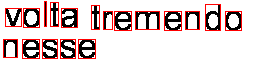
\includegraphics[scale=0.55]{./images/ocr.png}
        \end{center}
  \legend{ \small Fonte: Autor.}
\end{figure}


\begin{figure}[htb]
        \caption{\label{cascadia} \small Cacadia Code em negrito, com 10 de tamanho, 2 colunas e 5 blocos de texto. A entrada possue baixa resolução e ruídos. }
        \begin{center}
            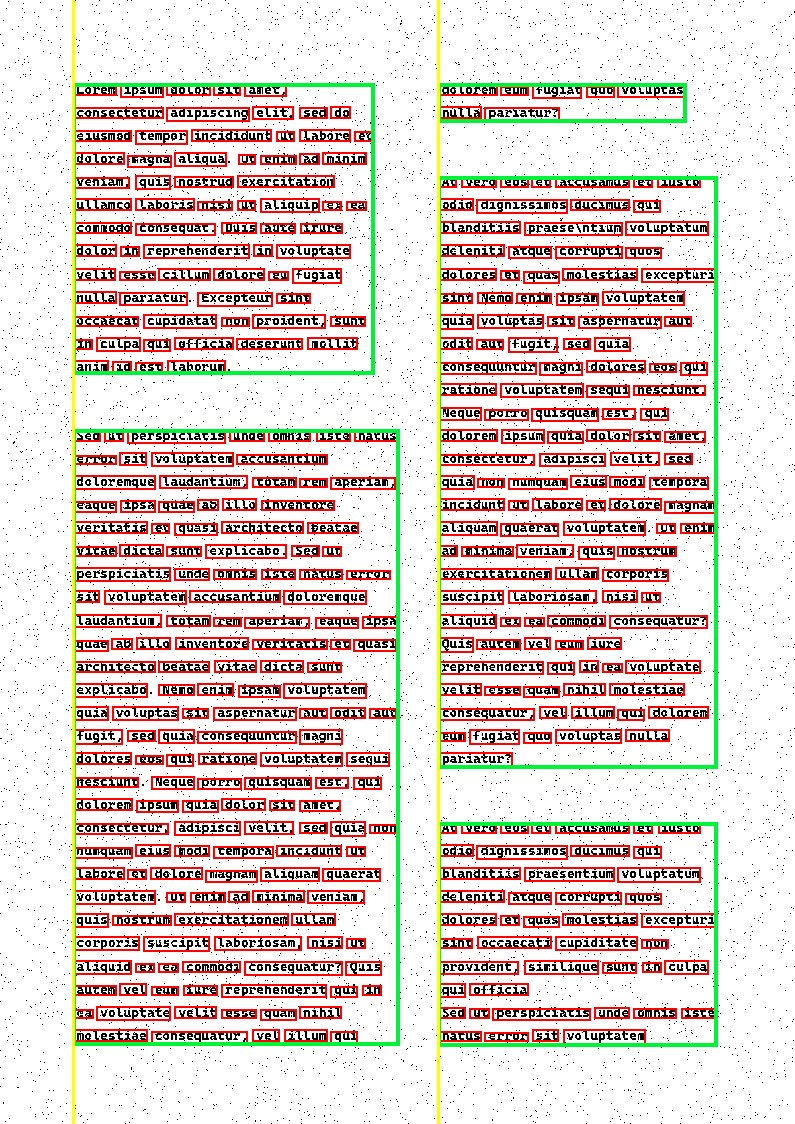
\includegraphics[scale=0.55]{./images/cascadia_code_10_detected_colunas_2_blocos_5_linhas_42_palavras_395.png}
        \end{center}
  \legend{ \small Fonte: Autor.}
\end{figure}

\begin{figure}[htb]
        \caption{\label{cascadia16} \small Cacadia Code centralizado, com 16 de tamanho, 2 colunas e 4 blocos de texto. }
        \begin{center}
            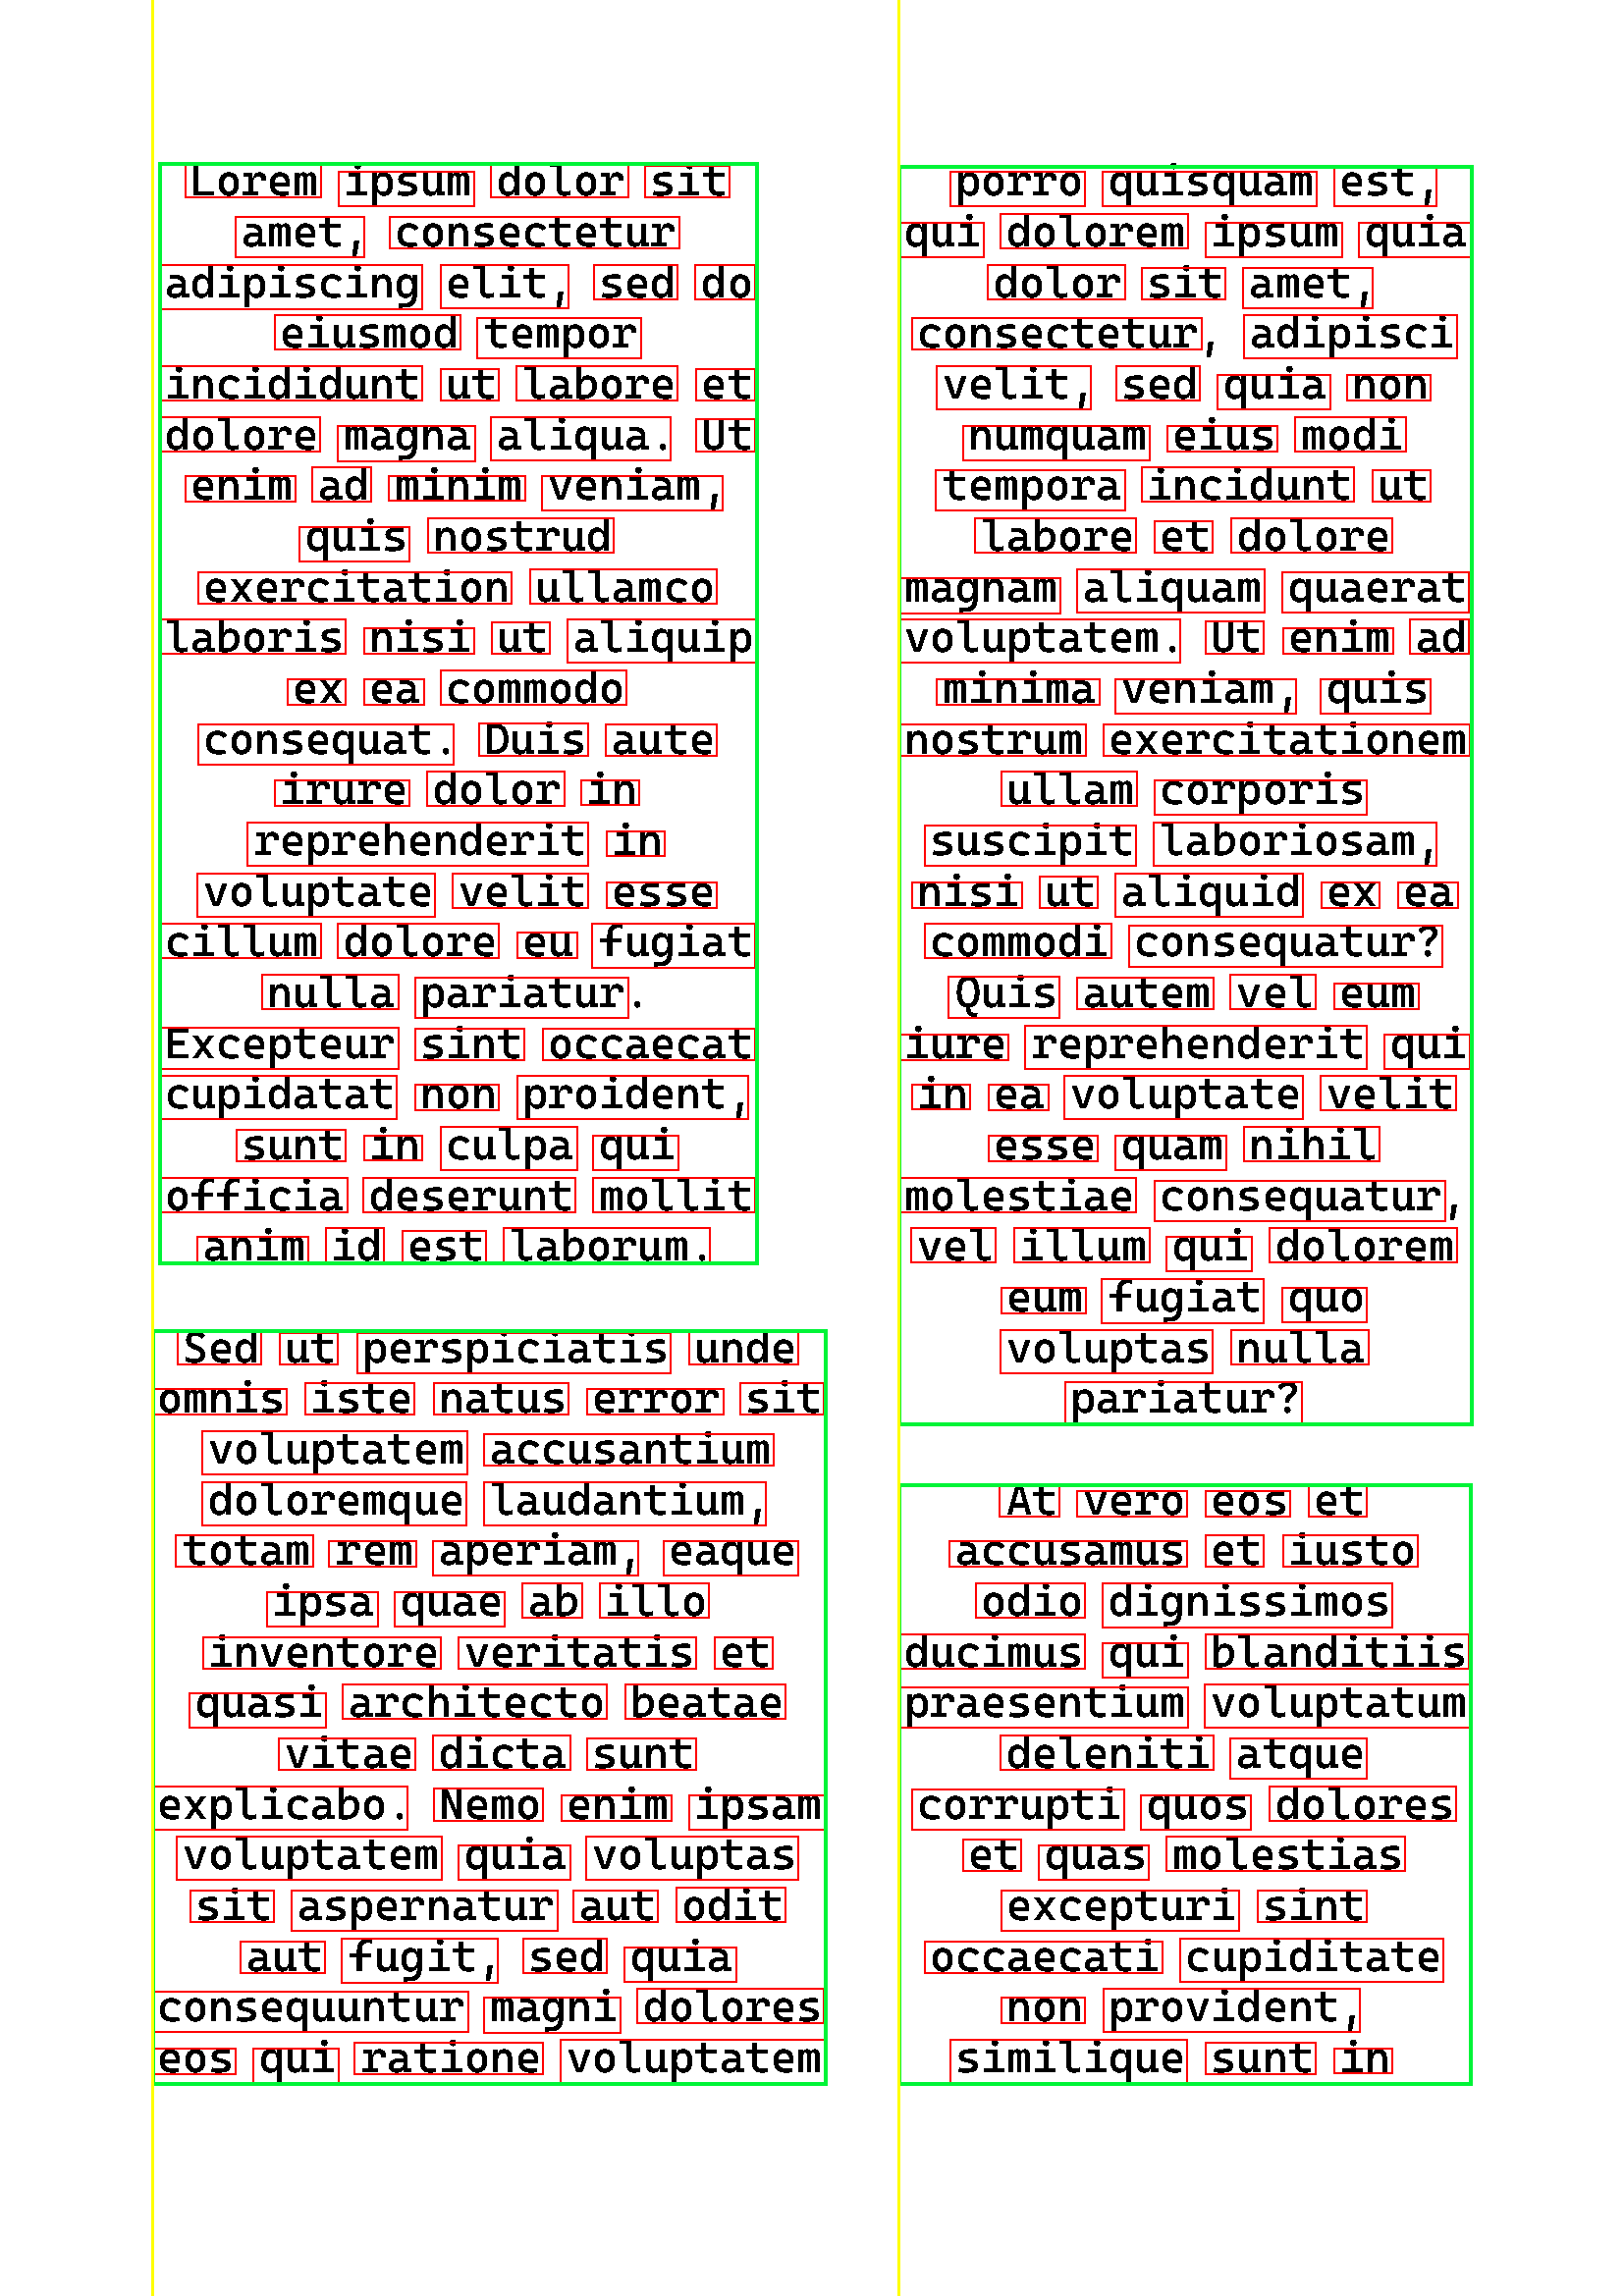
\includegraphics[scale=0.25]{./images/cascadia_code_centralizado_tamanho_16_colunas_2_blocos_4_linhas_38_palavras_226.png}
        \end{center}
  \legend{ \small Fonte: Autor.}
\end{figure}

\begin{figure}[htb]
        \caption{\label{timesnewroman} \small Times News Roman em itálico, com 18 de tamanho, com 4 colunas, 6 blocos de texto.}
        \begin{center}
        \end{center}
        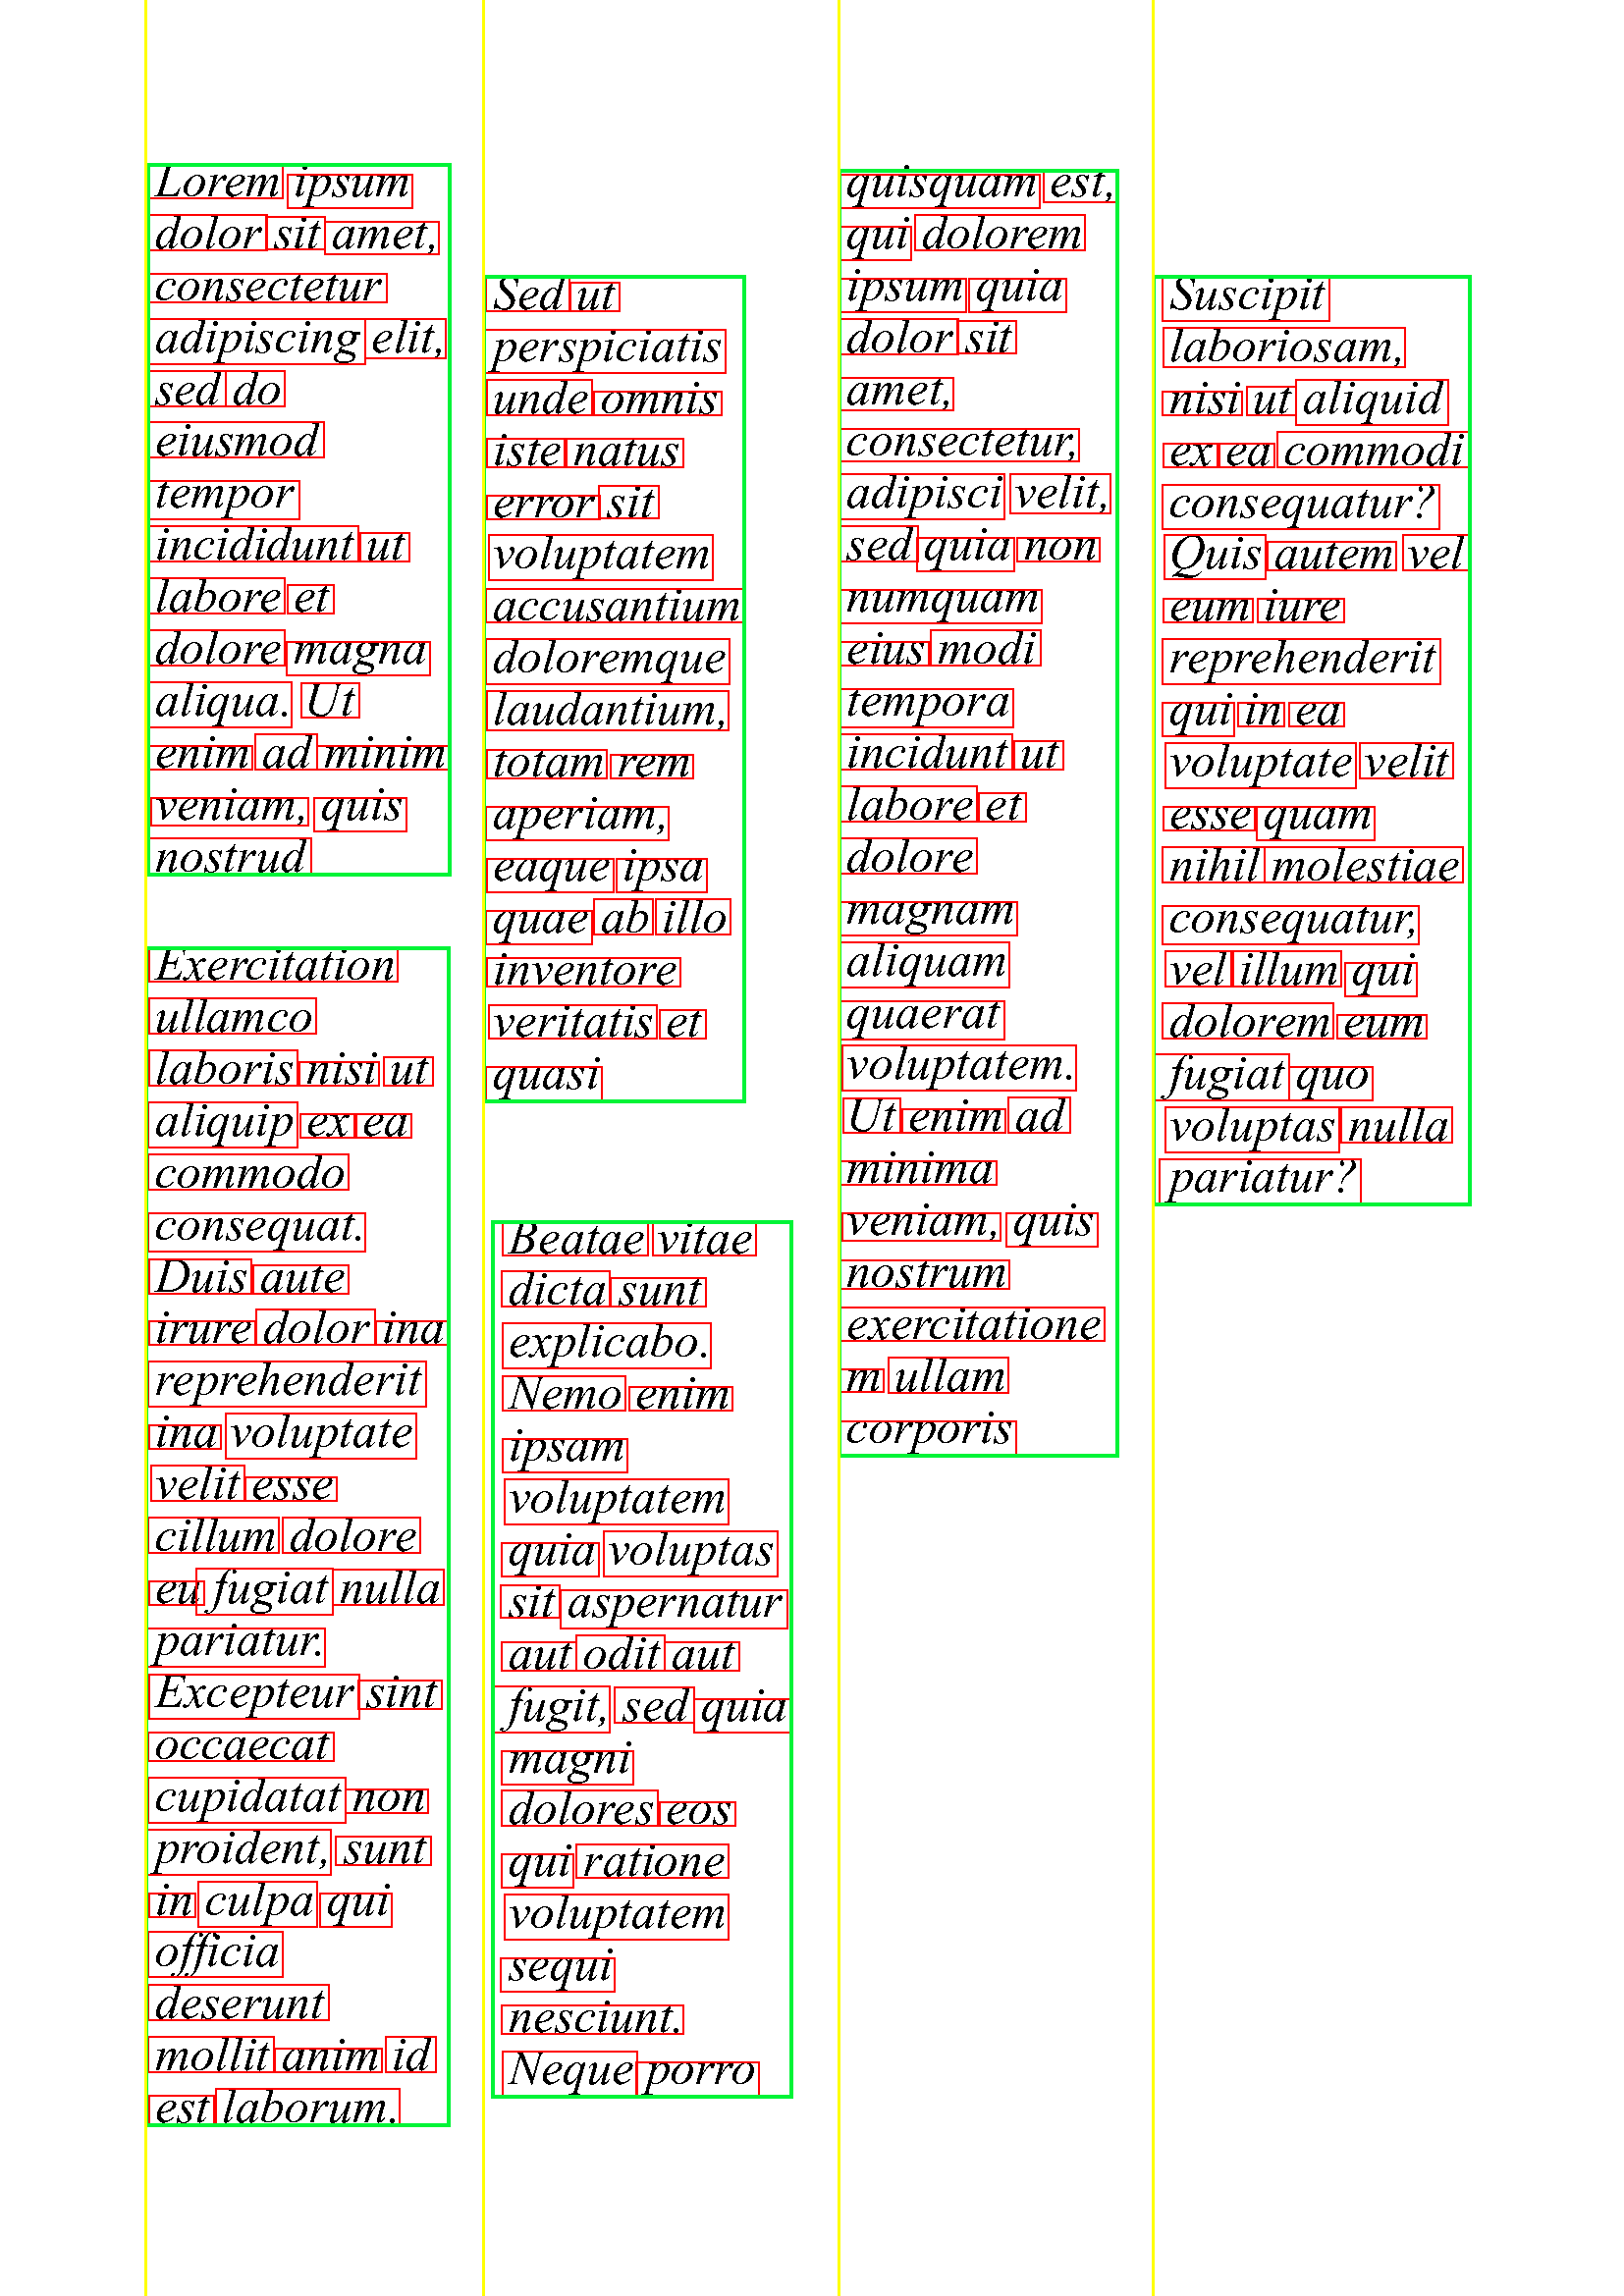
\includegraphics[scale=0.29]{./images/times_new_roman_colunas_4_blocos_6_linhas_38_palavras_197.png}
  \legend{ \small Fonte: Autor.}
\end{figure}


\begin{figure}[htb]
  % impact_esquerda_tamanho_40_colunas_2_blocos_2_linhas_18_palavras_46
        \caption{\label{impact} \small Impact com tamanho 40, 2 colunas e 2 blocos de texto. }
        \begin{center}
            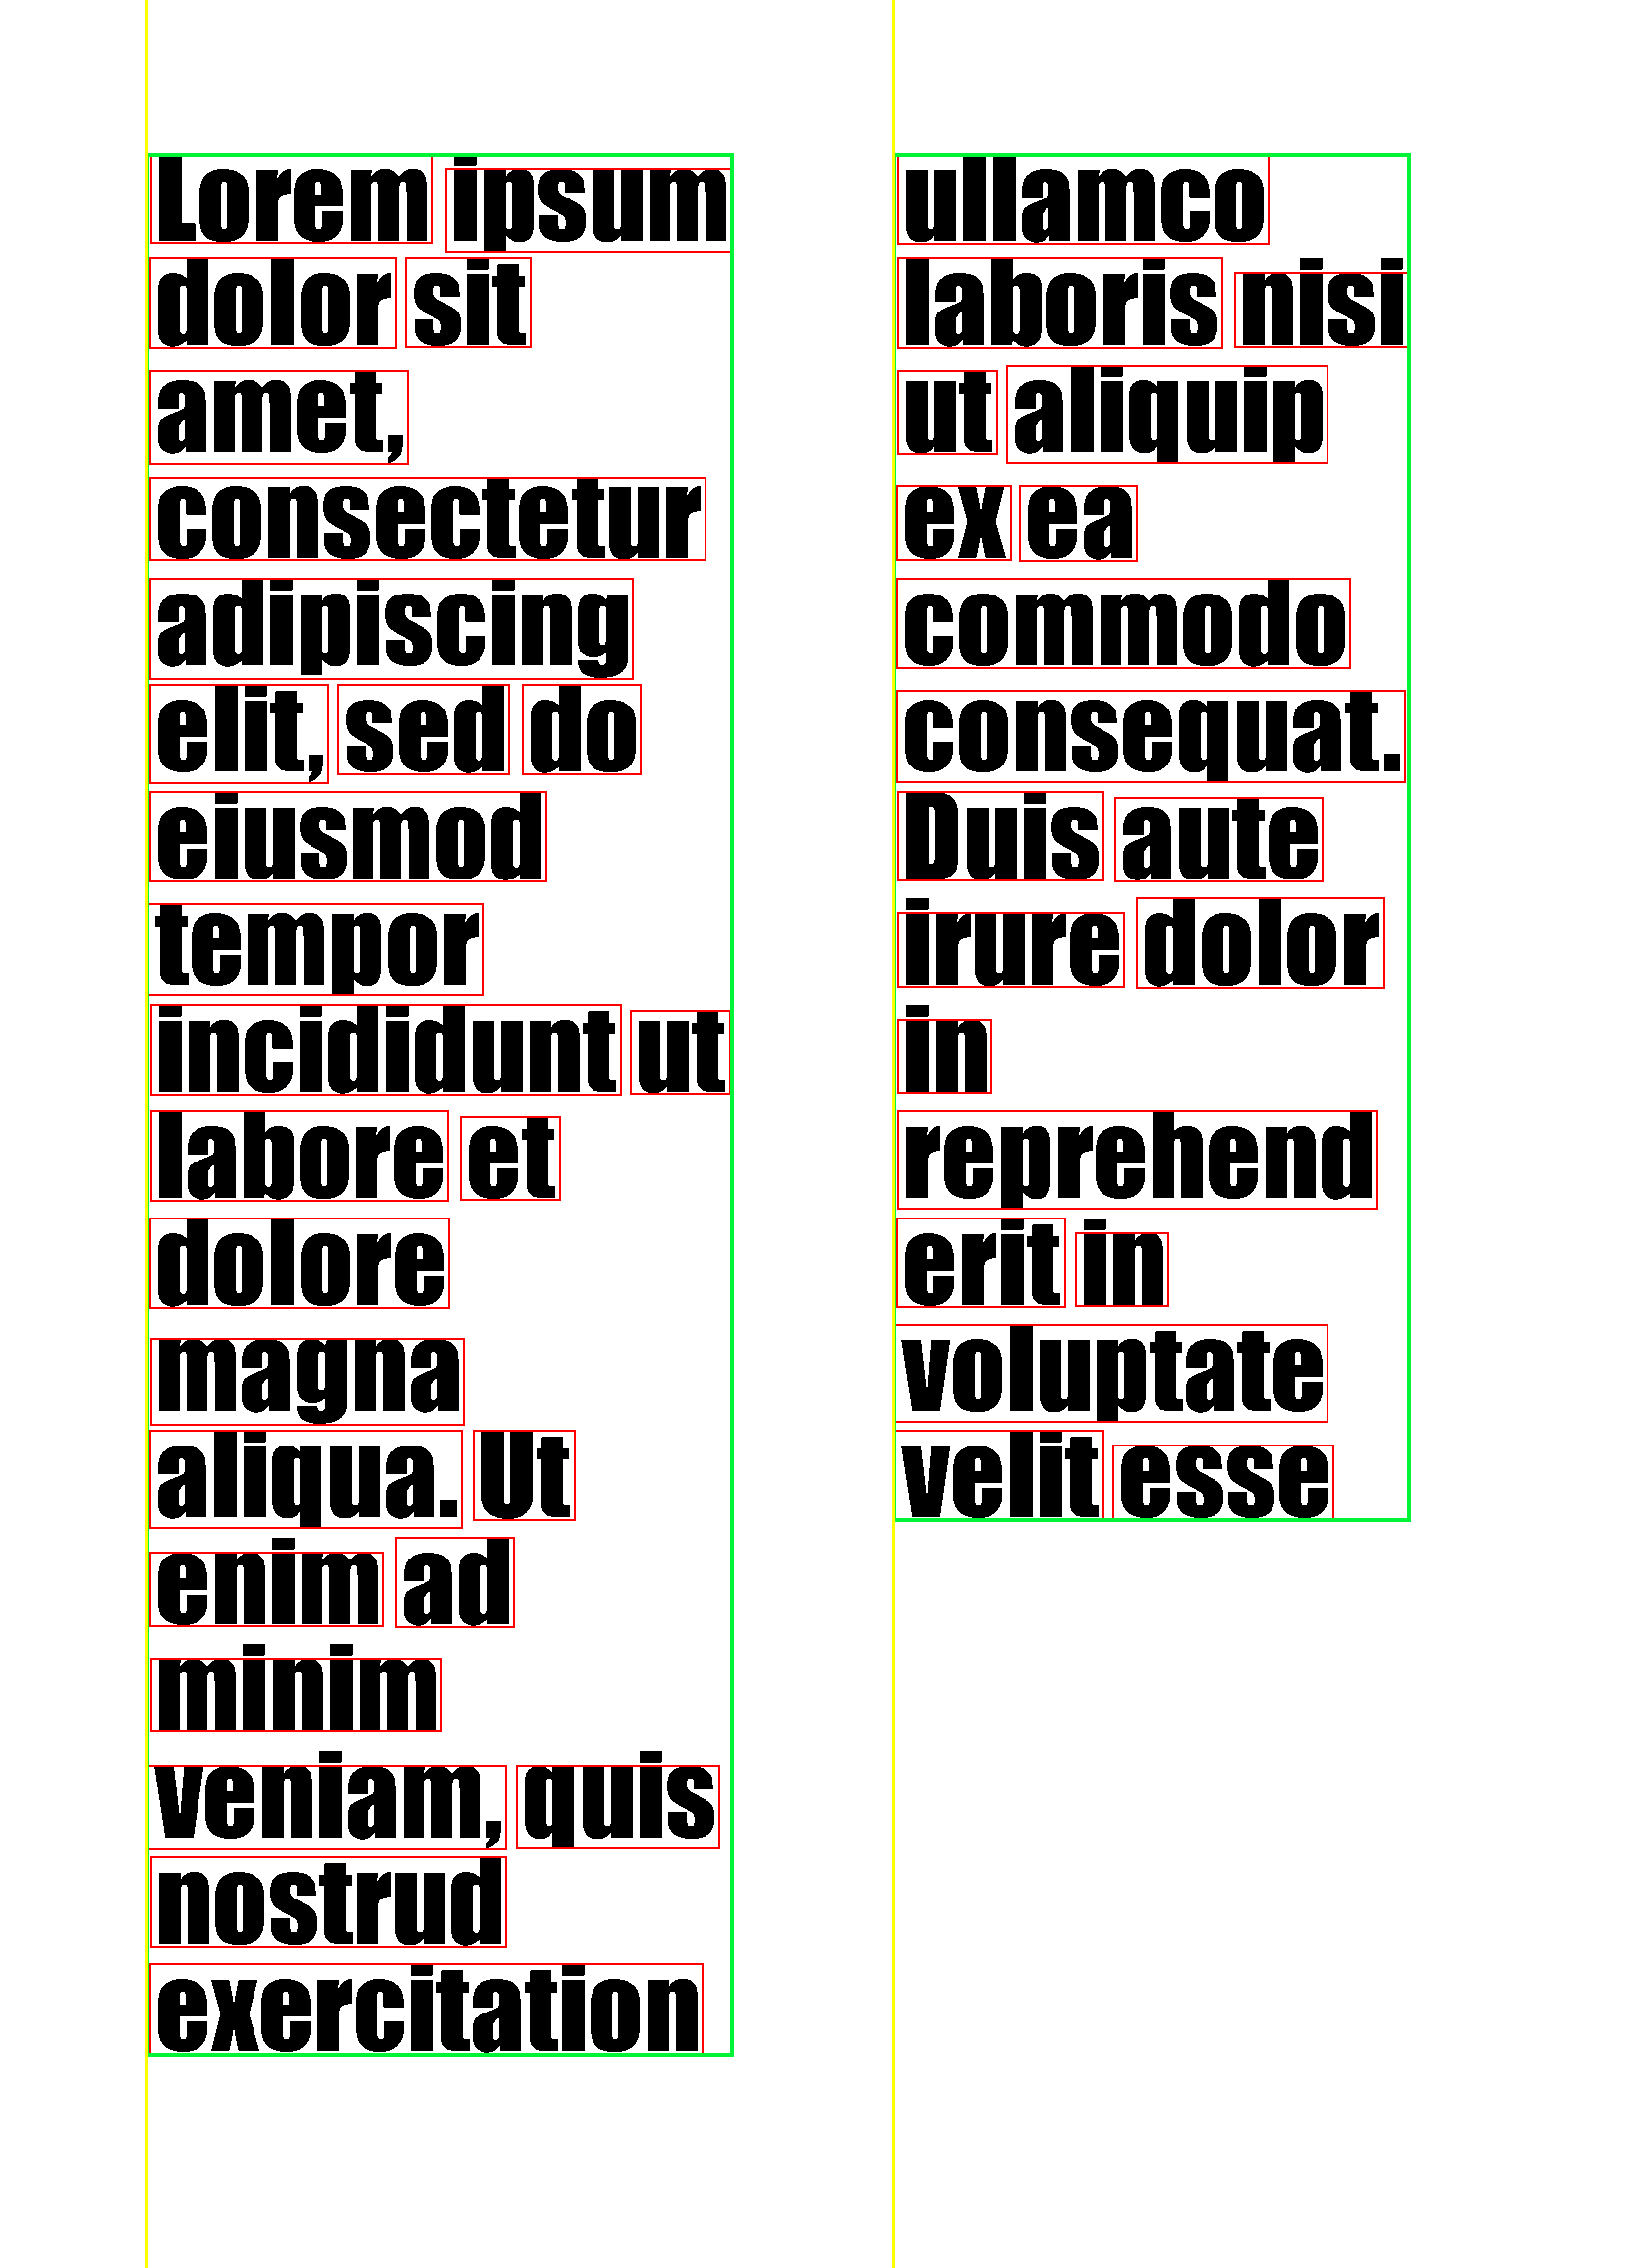
\includegraphics[scale=0.21]{./images/impact_columns.png}
        \end{center}
  \legend{ \small Fonte: Autor.}
\end{figure}

\begin{figure}[htb]
        \caption{\label{comic} \small Comic Sans centralizado, com 8 de tamanho, 2 colunas e 5 blocos de texto.}
        \begin{center}
            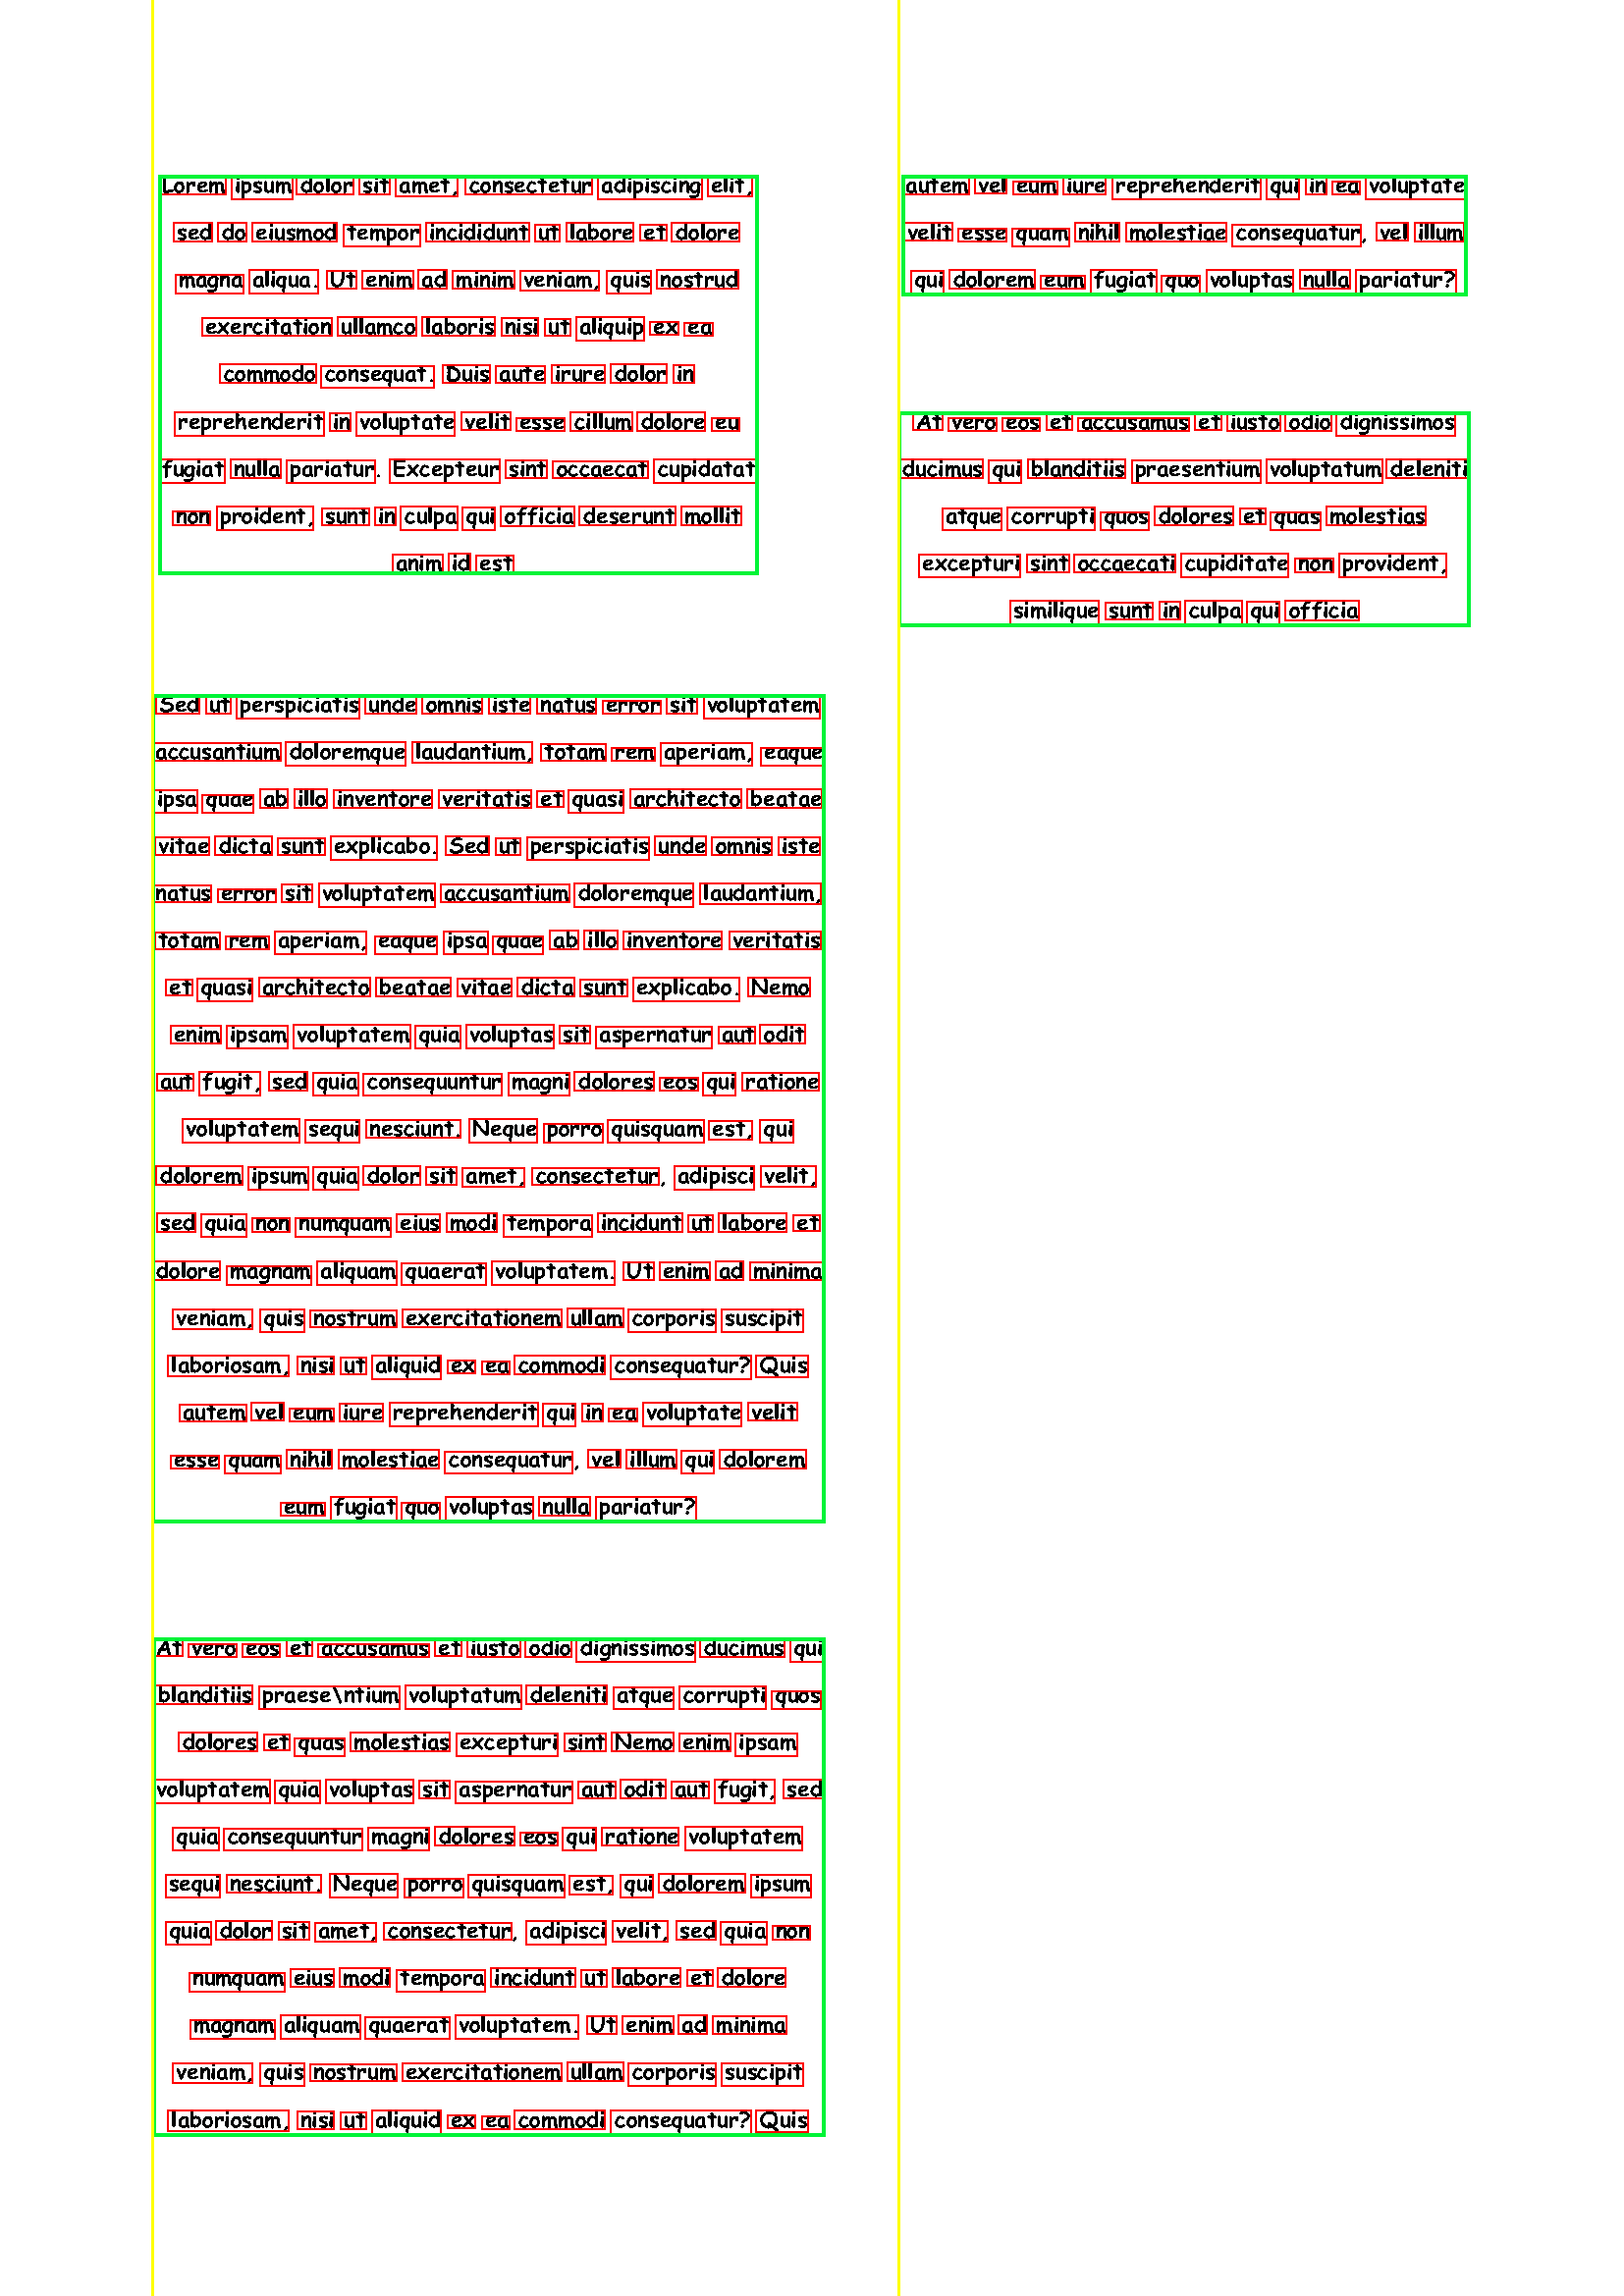
\includegraphics[scale=0.25]{./images/comic_sans_ms_bold_centralizado_tamanho_8_colunas_2_blocos_5_linhas_39_palavras_384.png}
        \end{center}
  \legend{ \small Fonte: Autor.}
\end{figure}

\begin{figure}[htb]
        \caption{\label{arial} \small Arial justificado, com 12 de tamanho, 3 colunas e 8 blocos de texto.}
        \begin{center}
            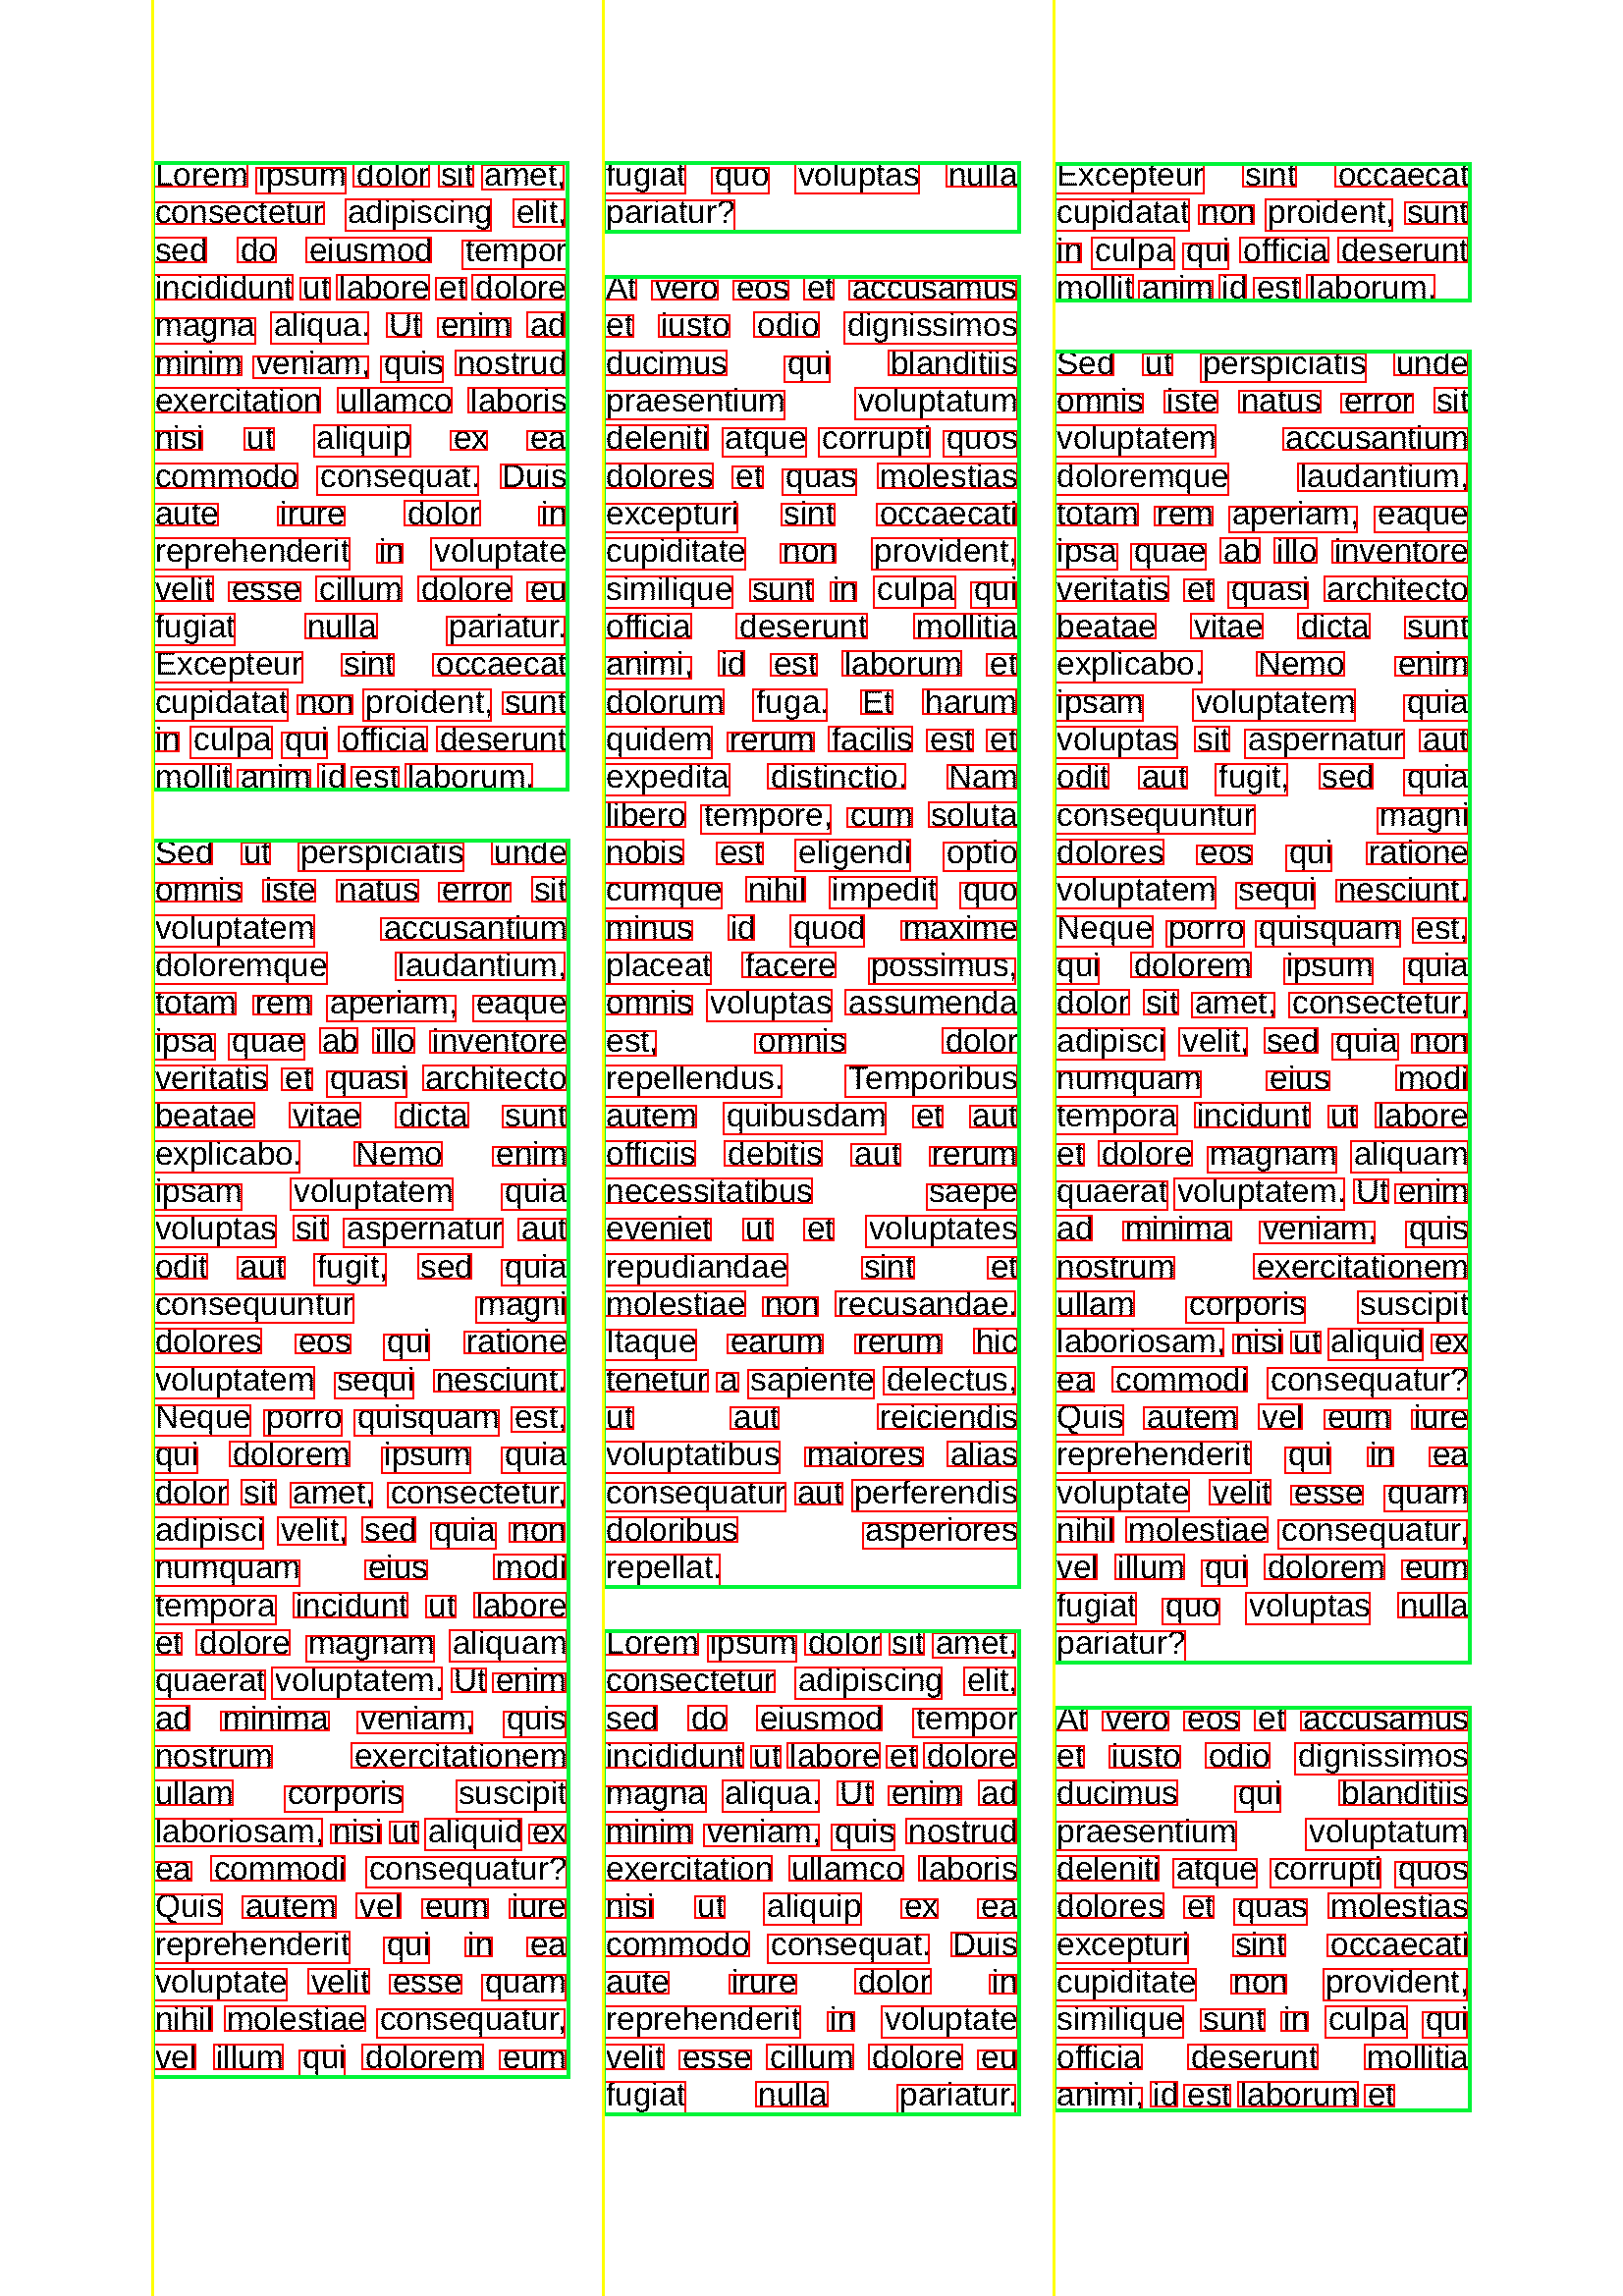
\includegraphics[scale=0.25]{./images/arial_justificado_tamanho_12_colunas_3_blocos_8_linhas_52_palavras_557.png}
        \end{center}
  \legend{ \small Fonte: Autor.}
\end{figure}


\chapter{Instruções \& Observações sobre o Projeto}
\label{ch-notas}

Primeiramente, certifique-se de ter baixado ``\texttt{.zip}'' ou clonado o repositório do projeto, o qual pode ser encontrado através do link \url{https://github.com/evertonse/pim}. Verifique se possui os requisitos listados na \autoref{sec-req}. Em seguida, na linha de comando, navegue até a pasta raiz do projeto e execute o seguinte comando, substituindo \texttt{caminho/para/imagem.pbm} pelo caminho da imagem que deseja processar:

\begin{verbatim}
$ python3 src/main.py caminho/para/imagem.pbm
\end{verbatim}

Exemplo de imagem usada pode ser:
\begin{verbatim}
$ python3 src/main.py assets/grupo_13_arial_esquerda_tamanho
_16_colunas_2_blocos_4_linhas_39_palavras_318.pbm
\end{verbatim}

\subsection{Formato das Imagems de Teste Criadas pelo Grupo}
Se nenhuma imagem for fornecida, será usada uma imagem padrão. Imagens de exemplo adicionais geradas pelo nosso grupo podem ser encontradas na pasta "\texttt{assets}". Essas imagens seguem o padrão adaptado do documento PreOCR, pois precisamos identificar mais detalhes sobre a imagem. Seja $F$, $T$, $C$, $B$, $L$ e $P$ variáveis que representam informações sobre a fonte (tipo) e se é justificado, centralizado, etc., tamanho, número de colunas, número de linhas, número de blocos e número de palavras, respectivamente. Assim, o nome das imagens de teste segue o padrão \texttt{grupo\_13\_F\_tamanho\_T\_colunas\_C\_blocos\_B\_linhas\_L\_palavras\_P}. Um exemplo é:

\begin{itemize}
  \item \texttt{\small grupo\_13\_arial\_esquerda\_tamanho\_16\_
    colunas\_2\_blocos\_4\_linhas\_39\_palavras\_318}.
\end{itemize}

\section{Requisitos} \label{sec-req}
\begin{itemize}
  \item É necessário ter o Python instalado para executar o script. A versão testada foi 3.10 e 3.11, mas possivelmente pega em versões superiores à 3.4
  \item Opcionalmente se a ferramenta \texttt{ffmpeg} for instalada e esteja disponível no caminho do sistema o projeto irá gerar vídeos. No Ubuntu, \texttt{ffmpeg} pode ser instalado usando \texttt{sudo apt install ffmpeg} ou \texttt{sudo snap install ffmpeg}.
  \item A biblioteca \texttt{numpy} é necessária para manipulação eficiente das matrizes (listas de pythons são absurdamente lentas). Foi instalado apenas pela estutura de dados. As operações usadas do numpy são bem simples:  multiplicação de matriz por escalar; tirar o maximo ou minimo de matrizes; soma e subtração de matrizes. Pode ser instalada via \texttt{pip install numpy}. Se o \texttt{pip} não estiver instalado, ele pode ser obtido executando \texttt{sudo apt install python3-pip} no Ubuntu. \end{itemize}

\section{Observações}


Todos os arquivos gerados durante a execução do projeto são armazenados na pasta "\texttt{output/}", com exceção do arquivo principal que contém os retângulos das palavras em vermelho e do arquivo de vídeo. Esses dois arquivos são prefixados com "\texttt{group\_13}" e estão localizados no diretório atual.
O site \href{https://convertio.co/pdf-pbm/}{convertio.co} foi usado para converter arquivos PDF para o formato PBM para arquivos de entrada adicionais. As pastas e seus conteúdos, ilustrados na \autoref{folders}, estão organizados da seguinte forma:

\begin{itemize}
\item \textbf{src/}: diretório que contém o código-fonte do projeto.
\item \textbf{src/kernels.py}: definição dos elementos estruturante.
\item \textbf{src/main.py}: arquivo principal do projeto contendo o código de execução principal.
\item \textbf{src/ocr.py}: implementação da detectção e da tentativa de reconhecimento óptico de caracteres.
\item \textbf{src/pim.py}: implementação das funções de processamento de imagens usadas: dilatação, erosão, filtro mediana.
\item \textbf{src/utils.py}: contém funções de utilidade como ler imagem, escrever imagem, fazer resize de imagem.
\item \textbf{assets/}: contém as imagem \texttt{.pbm} criados pelo grupo.
\item \textbf{assets/letters/}: contém os modelos de letras utilizados na tentativa de reconhecimento de caracteres.
\item \textbf{assets/professora/}: contém as imagem .pbm disponibilizados pela professora, mas com os nomes adaptados.
\item \textbf{output/}: local onde são armazenados os arquivos gerados durante a execução do projeto, sendo apenas os resultados intermediários.
\end{itemize}

\begin{figure}[htb]
\caption{\small Estrutura de pastas do projeto.}
\label{folders}
    \begin{center}
    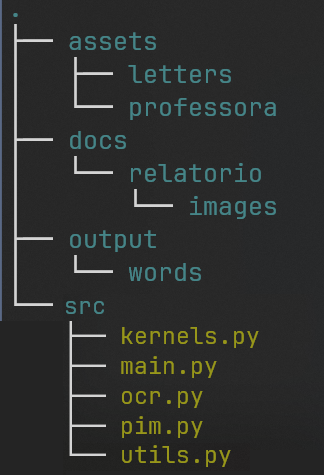
\includegraphics[scale=0.65]{./images/folders.png}
    \end{center}
\legend{ \small Fonte: Autor.}
\end{figure}

No exemplo de execução do projeto apresentado no \autoref{usage}, são fornecidas diversas informações úteis durante a execução do comando. Essas informações incluem o tempo decorrido para cada etapa do processamento, como a leitura do arquivo de imagem, aplicação de filtros, aplicação da dilatação, detecção de componentes conectados, criação do vídeo resultante, entre outros. Além disso, o nome do vídeo salvo e o nome do arquivo final gerado também são exibidos durante a execução do comando. O resultado final da execução, que inclui o número total de palavras, linhas, colunas e blocos detectados na imagem processada, é apresentado na última linha, prefixado com o caractere ''\texttt{>}``.

\begin{codigo}[h]
  \caption{\small Rodando o projeto na linha de comando.}
 \label{usage}
\begin{lstlisting}
USAGE: python3 src/main.py [path/to/image.pbm]

INFO: using default image path `./assets/grupo_13_cascadia_code_bold_esquerda_noisy
_tamanho_10_colunas_2_blocos_5_linhas_42_palavras_395.pbm`
INFO: read_ppm_file took 0.0697s to execute.
INFO: Image is 795x1124 (width x height).
INFO: fast_median_blur took 1.0870s to execute.
INFO: fast_dilate2 took 0.0114s to execute.
INFO: fast_dilate2 took 0.0142s to execute.
INFO: fast_dilate2 took 0.0073s to execute.
INFO: closing took 0.0171s to execute.
INFO: find_connected_components_bboxes took 0.7458s to execute.
INFO: choose_best_height took 0.0001s to execute.
INFO: median height found is 11 pixels.
INFO: group_bboxes took 1.6317s to execute.
INFO: wrote video output to `group_13_video.mp4`.
INFO: create_video_from_images took 2.9656s to execute.
INFO: wrote final output to `./group_13_detected_colunas_2_blocos_5_linhas_42_palavras_395.ppm`.

> 395 words, 42 lines, 2 columns, 5 blocks.
\end{lstlisting}
\end{codigo}


\chapter{Métodos, Parametros e Implementações}\label{ch-detalhes}

Neste trabalho, aplicamos técnicas de processamento de imagem para detecção e análise de palavras, linhas, colunas e blocos em documentos de texto. Para alcançar esse objetivo, utilizamos operações de dilatação e fechamento, juntamente com a detecção de componentes conectados, cujos parâmetros são especificados na \autoref{parametros}. Criamos elementos estruturantes personalizados para realizar operações específicas, como a detecção de palavras e a segmentação de blocos de texto. Além disso, para remoção de ruídos, aplicamos o filtro mediana. Implementamos também uma dilatação condicional da imagem, quando necessário, com base na altura média dos componentes conectados (palavras) já filtrados.

\section{Parâmetros} \label{parametros}
Nesta seção, apresentamos os parâmetros utilizados nos algoritmos, incluindo os elementos estruturantes de dilatação e fechamento, com diferentes tamanhos e formatos. Além disso, destacamos variáveis de limiar que são ajustadas para alterar o comportamento do algoritmo, adaptando-o às características da imagem sendo processada.

\begin{enumerate}
  \item Filtro Mediana: $3 \times 3$
  \item Primeira Dilatação: elemento estruturante horizontal truncada 5x5
\[
\begin{bmatrix}
0 & 0 & 0 & 0 & 0 \\
0 & 0 & 1 & 0 & 0 \\
0 & 1 & 1 & 1 & 1 \\
0 & 0 & 0 & 0 & 0 \\
0 & 0 & 0 & 0 & 0 \\
\end{bmatrix}
\]
  \item Fechamento: elemento estruturante para dilatação horizontal 3x3
\[
\begin{bmatrix}
0 & 0 & 0 \\
1 & 1 & 1 \\
0 & 0 & 0 \\
\end{bmatrix}
\]

  \item Dilatação Condicional: elemento estruturante para dilatação horizontal 5x5

\[
\begin{bmatrix}
0 & 0 & 0 & 0 & 0 \\
0 & 0 & 0 & 0 & 0 \\
1 & 1 & 1 & 1 & 1 \\
0 & 0 & 0 & 0 & 0 \\
0 & 0 & 0 & 0 & 0 \\
\end{bmatrix}
\]
       
\item Limiar para ocorrer dilatação condicional: altura mediana deve ser superior à 31 pixels.

\item Calculo da quantidade de iterações para dilatação condicional: \texttt{round}(1 + altura\_mediana / 31)

\item Componentes Conectados: consideramos 8-connectividade, isto é, as diagonais são consideradas conectadas.

\end{enumerate}


% Descrição das técnicas utilizadas para resolver o problema.
% Explicação de como as técnicas aprendidas na disciplina foram aplicadas.
% Parâmetros utilizados durante o processamento das imagens.

% Implementação:
% Inclusão de código-fonte relevante ou detalhes adicionais sobre a implementação, se necessário.


\section{Detalhes} 

O algoritmo inicia lendo a imagem de entrada e realizando pré-processamento, o qual inclui a aplicação do filtro da mediana (chamado de \texttt{median\_blur} no código) e a inversão das cores. Essas etapas têm como objetivo remover possíveis ruídos, como o ruído do tipo sal e pimenta, como ilustrado na \autoref{ruidos}. Como os ruídos são confirmados ter tamanho máximo de 1 pixel, um filtro $3 \times 3$ é suficiente. A inversão da imagem é realizada para facilitar a aplicação de algoritmos morfológicos, como a dilatação.

A dilatação é aplicada para melhorar a conectividade dos componentes de texto (palavras) na imagem. Dependendo dos parâmetros especificados, o algoritmo pode realizar operações adicionais, como fechamento (\texttt{closing}) ou abertura (\texttt{opening}), para refinar ainda mais as regiões de texto.

A abordagem do algoritmo envolve o uso de um elemento estruturante, conhecido como SE (\textit{Structuring Element}), para conectar as letras. Isso pode ser alcançado com um SE de formato horizontal. Embora tenham sido testados diferentes tipos de SE, como formatos circular, de cruz e vertical, o SE horizontal mostrou-se mais eficaz. Essa escolha é justificada pelo fato de que as letras normalmente estão alinhadas horizontalmente, exigindo uma expansão na direção horizontal para conectá-las, como ilustrado na \autoref{horz}.

% Inicialmente, o algoritmo lê a imagem de entrada e a pré-processa aplicando filtro da mediana (nome da função no código é \texttt{median\_blur}) e invertemos as cores. Essas etapas visam retirar possíveis ruídos do tipo sal de pimenta, ilustrado na \autoref{ruidos}. Já que foi confirmado que os ruídos não passam do tamanho de 1 pixel um filtro $3 \times 3$ é suficiente. A inversão da imagem é feita para aplicar algoritmos morfológicos, como a dilatação. A dilatação é feita para melhorar a conectividade dos componentes de texto. Dependendo dos parâmetros especificados, o algoritmo pode aplicar operações adicionais como fechamento (\texttt{closing}) ou abertura (\texttt{opening}) para refinar ainda mais as regiões de texto. A ideia é utilizar um elemento estruturante, conhecido como SE (do inglês, \textit{Structuring Element}), que connecte as letras; isso pode ser feito com um SE que seja horizontal. Foi testado com diferentes SEs, como fomarto circular, de cruz e vertical, mas o melhor é o horizontal. E faz sentido, pois as letras vem logo à direta da anterior, então para conecta-las precisamos esticar na horizontal para "grudar" uma na outra como ilustrado na \autoref{horz}. 

\begin{figure}[htb]
        \caption{\label{ruidos} \small  Remoção de ruído. }
        \begin{center}
            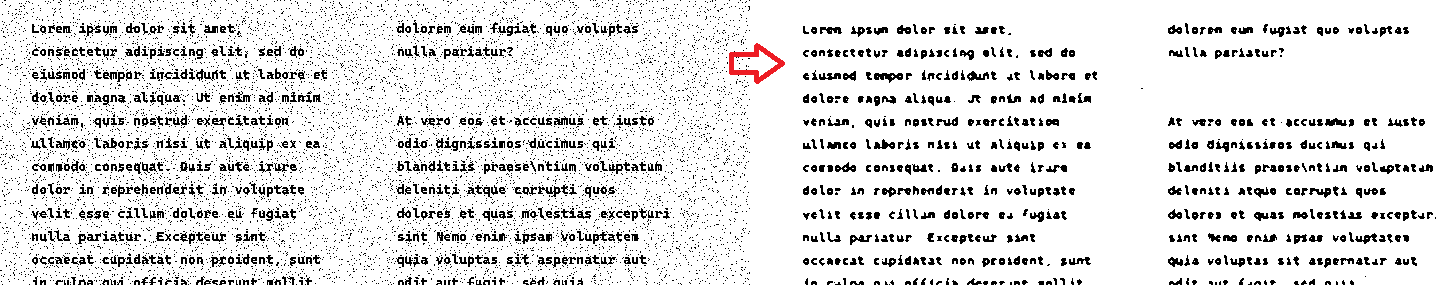
\includegraphics[scale=0.55]{./images/noise.png}
        \end{center}
  \legend{ \small Fonte: Autor.}
\end{figure}


\begin{figure}[htb]
        \caption{\label{horz} \small Resultado da aplicação de 2 iterações de dilatação com SE horizontal 5x5. }
        \begin{center}
            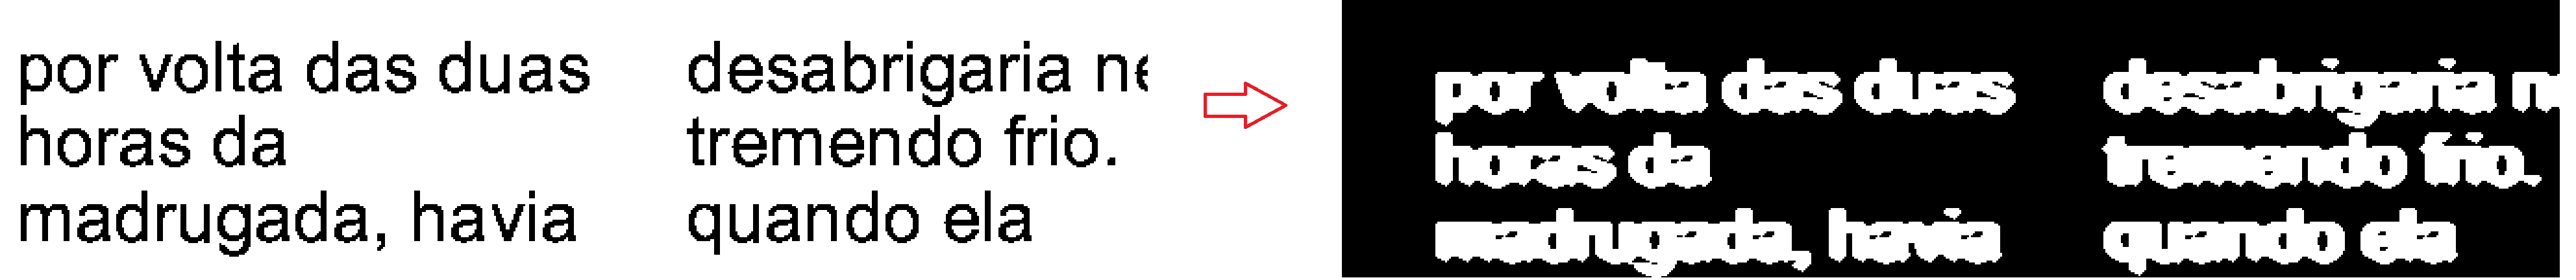
\includegraphics[scale=0.15]{./images/horizontal_5x5_aplicacao.png}
        \end{center}
  \legend{ \small Fonte: Autor.}
\end{figure}



\subsection{Componentes Conectados}


As operações de dilatação horizontal notavelmente aprimoraram a conectividade entre caracteres adjacentes na imagem. Esses conjuntos conectados de pixels representam as palavras individuais dentro da imagem. O conceito de componentes conectados é fundamentado em grafos e pode ser aplicado a imagens binárias, onde os pixels brancos correspondem aos nós. Existem diferentes tipos de conectividade. Se considerarmos apenas os vizinhos de um pixel como à esquerda, à direita, acima e abaixo, temos o que chamamos de 4-conectividade \cite[2.5.2 Adjacency, Connectivity, Regions, and Boundaries]{gonzalez2008digital}. Ao adicionar as diagonais, obtemos a 8-conectividade.

O algoritmo descrito no \autoref{cod-findcomp} identifica esses componentes conectados e se baseia em uma busca em profundidade, marcando os pixels visitados. A busca continua até que não haja mais caminhos a serem explorados na imagem, considerando também as diagonais, se \textit{connectivity} for igual 8). Quando não há mais caminhos a serem percorridos, o conjunto de pixels visitados forma um componente conectado. Esse processo é repetido até que todos os componentes tenham sido identificados, atualizando os pontos mais à esquerda inferior e mais à direita superior do componente, formando a \textit{bounding box} da palavra.

Em seguida, um retângulo é desenhado ao redor dessas palavras na imagem de saída. Opcionalmente, as palavras isoladas podem ser escritas em uma nova imagem, para uso posterior em tentativas de reconhecimento óptico de caracteres (OCR). Após a identificação dos componentes de texto, é realizada uma filtragem para eliminar as \textit{bounding boxes} correspondentes à pontuação (vírgulas, pontos) e manter apenas aquelas associadas às palavras.

O \autoref{cod-group_bboxes} ilustra como as palavras são então agrupadas em blocos com base em sua proximidade. A distância considerada é a menor diferença possível entre as duas \textit{bounding boxes}; se estiverem sobrepostas, então a distância é zero. Finalmente, a função \texttt{group\_bboxes} retorna a lista resultante, que contém todos os retangulos agrupados com base na distância máxima especificada; se a distância for maior, é considerado parte de outro grupo. Neste trabalho, essa distância máxima é encontrada de maneira dinâmica, executando o algoritmo uma vez para encontrar uma certa altura das palavras e, em seguida, executando novamente com essa informação adquirida. Para visualizar de forma interativa as etapas do algoritmo na descoberta desses blocos, é gerado um vídeo.


\begin{codigo}[h]
  \caption{\small Função para encontrar componentes conectados, considerando o tipo de conectividade.}
 \label{cod-findcomp}
\begin{lstlisting}[language=python]
def find_connected_components_bboxes(image, min_area=0, connectivity=8):
    nbrs = [(1, 0), (-1, 0), (0, 1), (0, -1)]
    if connectivity == 8:
        nbrs.extend([(1, 1), (1, -1), (-1, 1), (-1, -1)])

    def dfs(y, x):
        nonlocal nbrs, image
        min_y, min_x, max_x, max_y = y, x, y, x
        stack = [(y, x)]
        while stack != list():
            cy, cx = stack.pop()
            if (
                0 <= cy < image.shape[0]
                and 0 <= cx < image.shape[1]
                and not visited[cy, cx]
                and image[cy, cx] == 255
            ):
                visited[cy, cx] = True
                min_y = min(min_y, cy)
                min_x = min(min_x, cx)
                max_x = max(max_x, cy)
                max_y = max(max_y, cx)

                for dy, dx in nbrs:
                    stack.append((cy + dy, cx + dx))
        return min_y, min_x, max_x, max_y

    visited = np.zeros(image.shape, dtype=bool)
    bounding_boxes = list()

    for y in range(image.shape[0]):
        for x in range(image.shape[1]):
            if not visited[y, x] and image[y, x] == 255:
                min_y, min_x, max_x, max_y = dfs(y, x)
                bounding_boxes.append((min_y, min_x, max_x, max_y))

    return bounding_boxes

\end{lstlisting}
\end{codigo}

\begin{codigo}[h]
  \caption{\small Agrupamento dos retangulos.}
 \label{cod-group_bboxes}
\begin{lstlisting}[language=python]
def group_bboxes(bboxes, max_distance, image) -> list[list]:
    """
    Group bboxes based on a max distance.
    `image` is video for purposes
    """
    result = list()
    rest_idxs = [i for i in range(len(bboxes))]
    while len(rest_idxs) > 0:
        close_idxs = [rest_idxs.pop()]
        bbox = bboxes[close_idxs[0]]
        counter = 0
        while counter < len(rest_idxs):
            r_idx = rest_idxs[counter]
            counter += 1
            dist = distance(bbox, bboxes[r_idx])
            if (dist < max_distance) or bbox_overlap(bbox, bboxes[r_idx]):
                close_idxs.append(r_idx)
                rest_idxs.remove(r_idx)
                bbox = enclosing_bbox([bbox, bboxes[r_idx]])
                counter = 0

                vid_img = image.copy()
                y, x, y2, x2 = bbox
                rectangle(vid_img, (y, x), (y2, x2), (0, 244, 55), 2)
                video_frames.append(vid_img)

        y, x, y2, x2 = bbox
        rectangle(image, (y, x), (y2, x2), (0, 244, 55), 2)
        result.append([bboxes[i] for i in close_idxs])
    return result
\end{lstlisting}
\end{codigo}

\subsection{Detecção e Reconhecimento de Caracteres}


O processo de reconhecimento de caracteres é composto por três etapas principais: a detecção dos caracteres na imagem, a correspondência desses caracteres com os modelos predefinidos e o reconhecimento. Durante essa sequência, as \textit{bounding boxes} são geradas para cada caractere detectado. O \autoref{cod-ocr} mostra esse processo. Nele é carregado modelos de letras predefinidos no diretório \texttt{./assets/letters/}. Esses modelos são imagens binárias de letras individuais, como "v", "o", "l" e "t", com cada letra invertida para garantir que os pixels de interesse (brancos) tenham o valor 255 e os pixels de fundo (pretos) tenham o valor 0. A imagem a ser comparada é a subimagem que contém o caractere detectado; em seguida, as \textit{bounding boxes} são ordenadas da esquerda para a direita, seguindo a ordem de leitura.

Este recorte da letra é redimensionado para ter o mesmo tamanho das letras de referência. Para cada letra de referência, calcula-se a similaridade entre a letra recortada e o modelo. Essa similaridade é medida contando o número de pixels brancos iguais, na mesmas coordenadas nas duas imagens. A letra com a maior similaridade é considerada a melhor correspondência para a região.


\begin{codigo}[h]
  \caption{\small Função para reconhecimento de caracteres.}
 \label{cod-ocr}
\begin{lstlisting}[language=python]
# Package OCR
def string(img, letters):
    print(img.shape)
    orig = pim.convert_to_rgb(img)
    img = pim.invert(img)
    bbxs = pim.find_connected_components_bboxes(img, connectivity=8)
    # Start from leftmost
    bbxs = sorted(bbxs, key=lambda b: b[1])

    letter_sequence = []
    for b in bbxs:
        y, x, y2, x2 = b
        best_sim = 0
        best_letter = "-"
        for l, limg in letters.items():
            resized = pim.resize(img[y:y2, x:x2], *limg.shape)
            sim = 0
            for j in range(limg.shape[0]):
                for i in range(limg.shape[1]):
                    if resized[j, i] > 0:
                        if limg[j, i] > 0:
                            sim += 1
            if sim > best_sim:
                best_sim = sim
                best_letter = l
        letter_sequence.append(best_letter)

    return "".join(letter_sequence), orig
\end{lstlisting}
\end{codigo}





% Ao longo do processo, o algoritmo incorpora várias otimizações e ajustes de parâmetros para se adaptar a diferentes tipos de imagens de entrada e layouts de texto. Por exemplo, parâmetros como tamanho do kernel e contagens de iteração são ajustados dinamicamente com base nas características da imagem de entrada, como tamanho do texto e níveis de ruído.

\subsection{Operações Morfológicas}
\subsubsection{Dilatação}

 A dilatação morfológica é útil para preencher pequenos espaços entre objetos. No \autoref{udilate}, a função `understandable\_dilate` implementa a dilatação de forma "compreensível", mais compativel com a definição dada em \citeonline[9.2.2 Dilation]{gonzalez2008digital}.

 Nessa implementação a variável \texttt{kernel} representa o elemento estruturante, que define a forma e o tamanho da dilatação. Durante o processo, a imagem é percorrida pixel a pixel, e para cada pixel, verifica-se se pelo menos um dos pixels na vizinhança definida pelo kernel é branco (valor 255). Se pelo menos um dos pixels na vizinhança é branco, o pixel central é definido como branco (255) na imagem resultante. Caso contrário, o pixel central é definido como preto (0).

 Uma interepretação util é que o elemento estruturante define qual é a vizinhaça, onde tiver 1 no elemento indica que faz parte da vizinhaça, se tiver zero então não faz parte. Para cada x,y percorridos a imagem resultado é o máximo o valor de sua vizinhança definido pelo elemento estruturante.

\begin{codigo}[h]
  \caption{\small Dilatação.}
 \label{udilate}
\begin{lstlisting}[language=python]
def understandable_dilate(image, kernel):
    result = np.zeros(image.shape)
    height = image.shape[0]
    width = image.shape[1]
    kernel_height = kernel.shape[1]
    kernel_width = kernel.shape[0]
    kernel_width_delta = kernel_width // 2
    kernel_height_delta = kernel_height // 2
    for y in range(height):
        for x in range(width):
            all_good = False
            for j in range(kernel_height):
                for i in range(kernel_width):
                    i_offset = i - kernel_width_delta
                    j_offset = j - kernel_height_delta
                    color = 0
                    if (
                        (x + i_offset) >= 0
                        and (x + i_offset) < width
                        and y + j_offset >= 0
                        and y + j_offset < height
                    ):
                        color = image[y + j_offset, x + i_offset]
                    kcolor = kernel[j, i]
                    if int(kcolor) * int(color):
                        all_good = True
                        break
                if all_good:
                    break
            if all_good:
                result[y, x] = 255
            else:
                result[y, x] = 0
    return result
\end{lstlisting}
\end{codigo}

  % Professora Bia, aqui eu disponho diferentes implementações de dilatação
  % understandable_dilate é o mais lento que tenta ser o mais entendivel possivel.
  % Ja fast_dilate2 é bem mais rapido, porém usa a função `maximum` da estrutura de dados matrix do  numpy.
  % é uma função que como o nome diz pega o maximo entre valores, mas funciona para matrix.
  % Eu dispus dessa maneira pra mostra que sei fazer todas as diferentes implementações,
  % mas pra ficar mais rapido e interativo é usado o fast_dilate2.
  % NOTE: Qualquer uma dessas implementações funciona para os propositos deste trabalho
No \autoref{fdilate2}, a função \texttt{fast\_dilate2} implementa uma dilatação morfológica mais rápida, aproveitando as operações de matriz do NumPy. A imagem é expandida com um preenchimento adequado para evitar problemas de borda durante a aplicação (o elemento estruturante é chamado de \texttt{kernel} no código). Em seguida, usando a função \texttt{np.maximum}, calculamos o valor máximo elemento a elemento da matriz entre a imagem resultante e o subconjunto da imagem com padding.

Inicialmente, a imagem resultante é preenchida com entradas zeradas e, à medida que iteramos sobre a altura $j$ e a largura $i$ do elemento estruturante, aplicamos essa função \texttt{maximum} em um  \textbf{subconjunto diferente} da imagem com \textit{padding}, dependendo de $j$ e $i$ atual. Isso é feito apenas se o elemento estruturante for maior ou igual a 1 na altura $j$ e largura $i$. Isso efetivamente realiza uma dilatação, onde o pixel central de uma vizinhança é definido como o valor máximo dessa vizinhança. No entanto, observe que a vizinhança depende do elemento estruturante, apenas onde os valores são 1 são considerados vizinhança.

\begin{codigo}[h]
  \caption{\small Ditalação mais rápida, usando operação de matriz.}
 \label{fdilate2}
\begin{lstlisting}[language=python]
def fast_dilate2(image, kernel):
    global counter 
    height, width = image.shape
    kernel_height, kernel_width = kernel.shape

    kernel_width_delta = kernel_width // 2
    kernel_height_delta = kernel_height // 2

    # We pad by the kernel delta, top, bottom, left and right
    padded_image = pad(
        image,
        kernel_height_delta,
        kernel_height_delta,
        kernel_width_delta,
        kernel_width_delta,
    )

    dilated = np.zeros(image.shape, dtype=np.uint8)
    for j in range(kernel_height):
        for i in range(kernel_width):
            if kernel[j, i] == 1:
                shifted_sub_image = padded_image[j : j + height, i : i + width]
                dilated = np.maximum(
                    dilated, shifted_sub_image
                )

    return dilated
\end{lstlisting}
\end{codigo}

Ambas as implementações alcançam o mesmo resultado de dilatação morfológica, mas \texttt{fast\_dilate2} é mais eficiente devido ao uso de operações vetorizadas do NumPy. Isso resulta em uma execução mais rápida, especialmente em imagens grandes.


\subsubsection{Erosão}

A erosão segue o mesmo princípio da dilatação, mas com a operação sendo o \texttt{mínimo} no lugar do \texttt{máximo}. A iteração começa com a imagem resultante tendo todas as entradas definidas como 1 em vez de 0. Na versão \texttt{understandable} da erosão, apenas quando \textbf{todos os pixels} da imagem se alinham com o elemento estruturante é que o pixel central é definido como 1 no lugar de \textbf{pelo menos um}. Vale ressaltar que a erosão não é necessária para o funcionamento do projeto, pois mesmo sem \texttt{closing} ou \texttt{opening}, que usam implicitamente a erosão, o algoritmo é robusto para os casos de teste mencionados na introdução. A função \texttt{opening} é a operação de abertura, que consiste em primeiro realizar uma erosão seguida de uma dilatação. É útil para remover pequenos ruídos e separar objetos próximos, mas neste trabalho, removemos esses ruídos através do filtro da mediana.


\subsubsection{Filtro Mediana}

O \autoref{cod-mediana} implementa um filtro de mediana. Ele percorre cada pixel da imagem e substitui o valor do pixel pela mediana dos valores dos pixels em sua vizinhança, definida pelo tamanho do filtro. Isso ajuda a remover ruídos e detalhes pequenos.

\begin{codigo}[h]
  \caption{\small Implementação do filtro de mediana.}
 \label{cod-mediana}
\begin{lstlisting}[language=python]
def understandable_median_blur(image, filter_size=3):
    assert len(image.shape) == 2

    result = image.copy()
    height = image.shape[0]
    width = image.shape[1]
    for y in range(height):
        for x in range(width):
            colors = list()
            for j in range(filter_size):
                for i in range(filter_size):
                    i_offset = i - filter_size // 2
                    j_offset = j - filter_size // 2

                    color = 0
                    if (
                        (x + i_offset) >= 0
                        and (x + i_offset) < width
                        and y + j_offset >= 0
                        and y + j_offset < height
                    ):
                        color = image[y + j_offset, x + i_offset]
                    colors.append(color)
            colors.sort()
            result[y, x] = colors[(len(colors) // 2)]
    return result
\end{lstlisting}
\end{codigo}

\subsubsection{Contagens}

A contagem de linhas, proposto no \autoref{cod-linecount}, verifica se a lista de caixas delimitadoras está vaziam, depois as \textit{bounding boxes} ordenadas verticalmente com base na coordenada y. Para cada \textit{bounding box}, calcula-se a sobreposição vertical com a anterior. Se a sobreposição for menor que uma fração mínima, contamos uma nova linha. Na \autoref{fig-linecount}, temos uma represetação do retangulo da linha em uma dada iteração desse algoritmo.

O algoritmo para contar colunas (\autoref{cod-columncount}) é semelhante ao de linhas, mas agora classificamos os retangulo horizontalmente em vez de verticalmente. Para cada retângulo ordenado, verificamos se sua coordenada x do canto inferior esquerdo é maior do que a coordenada x do canto inferior direito da caixa mais à direita encontrada até o momento (\texttt{max\_right}). Se for, consideramos isso como o início de uma nova coluna. Além disso, desenhamos uma linha vertical indicando o início da nova coluna na imagem de vídeo.

\begin{codigo}[h]
  \caption{\small Contagem de linhas.}
 \label{cod-linecount}
\begin{lstlisting}[language=python]
def count_lines(bboxes, orig):
    if len(bboxes) == 0:
        return 0
    bboxes = sorted(bboxes, key=lambda bbox: (bbox[0], bbox[2]))

    lines = 1
    prev1, _, prev2, _ = bboxes[0]
    xdiffs_bboxes = list()
    for bbox in bboxes[1:]:
        y1, _, y2, _ = bbox
        overlap = max(0, min(prev2, y2) - max(prev1, y1))
        if overlap > abs(prev1 - prev2) / 100:
            continue
        lines += 1
        prev1 = y1
        prev2 = y2

    return lines
\end{lstlisting}
\end{codigo}


\begin{figure}[htb]
        \caption{\label{fig-linecount} \small Frame do video mostrando o que o algortimo conta como linha. }
        \begin{center}
            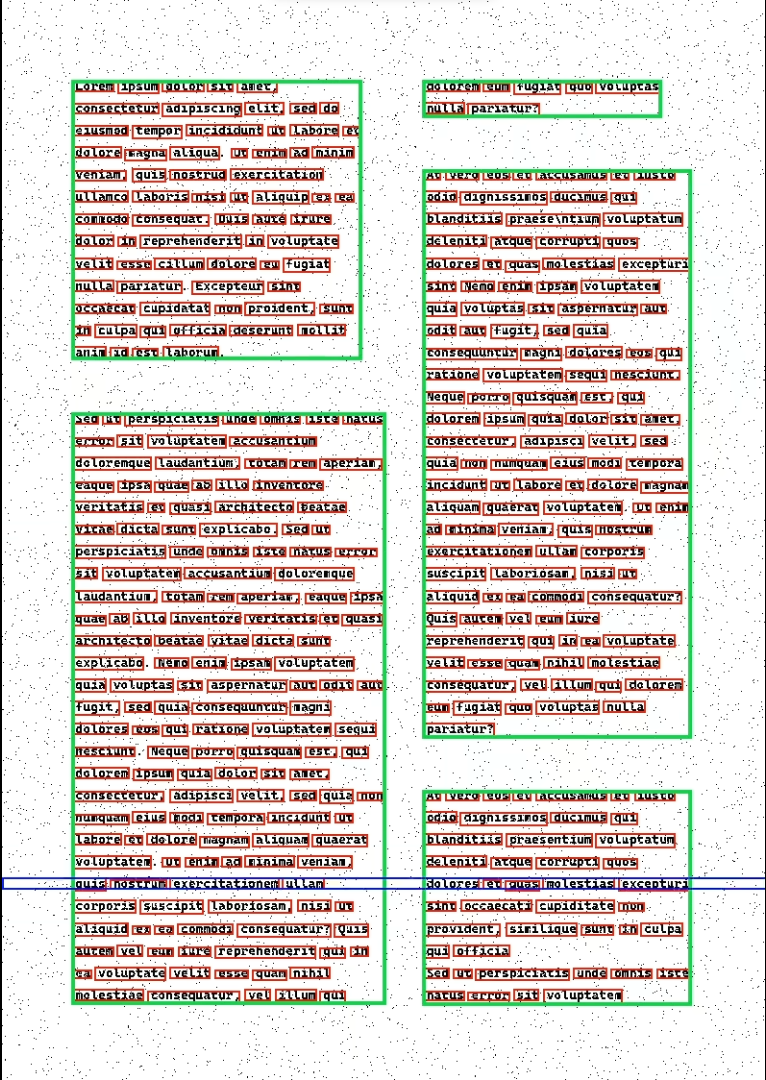
\includegraphics[scale=0.55]{./images/cascadia_line.png}
        \end{center}
  \legend{ \small Fonte: Autor.}
\end{figure}

\begin{codigo}[h]
  \caption{\small Contagem de colunas.}
 \label{cod-columncount}
\begin{lstlisting}[language=python]
def count_columns(bboxes, orig):
    # Sort by left x-coordinate
    sorted_bboxes = sorted(bboxes, key=lambda bbox: bbox[1])

    num_columns = 0
    max_right = float("-inf")

    for bbox in sorted_bboxes:
        _, left, _, right = bbox

        # If the left x-coordinate of the bounding box is greater than the current rightmost x-coordinate,
        # it indicates the start of a new column
        if left > max_right:
            num_columns += 1

        # Update current rightmost x-coordinate
        if max_right < right:
            max_right = right
    return num_columns
\end{lstlisting}
\end{codigo}




\chapter{Conclusão} \label{ch-conclusao}

Com base nos resultados obtidos, é possível afirmar que o desempenho do nosso algoritmo foi bastante satisfatório. Ele se mostrou eficaz para diversas fontes e tamanhos de texto, independentemente de estarem justificados, centralizados, alinhados à direita ou à esquerda. Além disso, funcionou igualmente bem com imagens de resoluções variadas, tanto baixas quanto altas, demonstrando uma boa robustez. A utilização do filtro da mediana mostrou-se suficiente para lidar com uma quantidade considerável de ruído na imagem. A estratégia de realizar a dilatação horizontal foi uma sacada importante que contribuiu significativamente para a melhoria da conectividade entre os caracteres.

A abordagem de utilizar alturas encontradas como heurística para decidir se novas operações morfológicas deveriam ser aplicadas também se mostrou eficaz, ampliando a capacidade do algoritmo de lidar com diferentes casos. No entanto, há espaço para explorar ainda mais heuristicas, como usar a distância média entre caracteres como limiar para decidir sobre a aplicação de operações de fechamento, ou estudar o espaço em branco entre as palavras. Uma outra possibilidade seria considerar uma porcentagem do tamanho das letras em relação à imagem inteira para tomar decisões.

Embora a detecção de caracteres tenha funcionado bem, o método de \textit{template matching} não teve o mesmo desempenho. Esse aspecto merece uma investigação mais aprofundada para entender por que não foi eficaz para reconhecer os caracteres (deu muitas similaridades erradas). No entanto, mesmo com esse desafio, o projeto como um todo foi capaz de realizar uma série de tarefas interessantes e diversas, incluindo a criação de um vídeo para visualização das etapas do algoritmo e a implementação de algoritmos vetorizados, proporcionando um entendimento mais profundo e intuitivo desses processos morfológicos.

\phantompart
\bibliography{Bibliografia}


%%%%%%%%%%%%%%%%%%%%%%%%%%%%%%%%%%%%%%%%%%%%%%%%%%%%%%
% ELEMENTOS PÓS-TEXTUAIS
%%%%%%%%%%%%%%%%%%%%%%%%%%%%%%%%%%%%%%%%%%%%%%%%%%%%%%


\postextual


\renewcommand{\chapnumfont}{\chaptitlefont}
\renewcommand{\afterchapternum}{}
% \include{Pos_Textual/Apendices}
% \include{Pos_Textual/Anexos}


\end{document}
